Dopo un accurato studio si è stipulata una lista di casi d'uso presentata qui di seguito. Ognuno dei quali è riportato come specificato nel documento \NdP, nel punto 2.2.3.1.4.
\subsection{Attori dei casi d'uso}
\subsubsection{Attori primari}
  \begin{enumerate}
      \item Utente non autenticato: utente il quale accede alla piattaforma sprovvisto di un account personale sulla piattaforma e/o che non esegue l'operazione di login;
      \item Utente autenticato: utente in possesso di un account personale sulla piattaforma e che ha eseguito con successo l'operazione di login.
  \end{enumerate}
  
 \subsubsection{Attori secondari}
 \begin{enumerate}
     \item Aws;
     \item Facebook.
 \end{enumerate}
    
    
\subsection{Elenco dei casi d'uso}
   \subsubsection{UC 1-Breve presentazione all'uso dell'applicazione}
  
   
    \begin{itemize}
        \item \textbf{Attori primari}: Utente non autenticato;
        \item \textbf{Scopo e descrizione}: L'utente visualizza una guida di introduzione che spiega brevemente le funzionalità che l'app possiede. Eventualmente l'utente se non interessato può decidere di interrompere la visualizzazione della guida; 
        \item \textbf{Scenario principale}: L'utente non autenticato, dopo aver aperto l'applicazione visualizza la guida introduttiva di presentazione;
        \item \textbf{Precondizione}: Il sistema è funzionante e l'utente sprovvisto di account che ha appena scaricato l'applicazione vi entra;
        \item \textbf{Postcondizione}: L’utente ha  avuto delle nozioni riguardanti le funzionalità dell'applicazione oppure ha deciso di saltare parte della guida introduttiva.
    \end{itemize}
    
  

        \subsubsection{UC 2-Registrazione}
        \begin{itemize}
        \item \textbf{Attori primari}: Utente non autenticato;
        \item \textbf{Attori secondari}: Aws;
        \item \textbf{Scopo e descrizione}: L'utente desidera creare il proprio profilo personale all'interno della piattaforma; 
        \item \textbf{Scenario principale}:
            \begin{itemize}
                \item L'utente non autenticato accede alla piattaforma;
                \item L'utente che desidera registrare il proprio account seleziona la funzionalità "Registrati";
                \item L'utente inserisce le credenziali richieste per creare un account;
                \item L'utente conferma la registrazione.
            \end{itemize}
        \item \textbf{Scenario secondario}: L'utente non intende proseguire con l'operazione di registrazione: interrompe l'inserimento dei dati e la registrazione non viene effettuata.
        
        
        
        
        \item \textbf{Precondizione}: L'utente non è riconosciuto nel sistema;
        \item \textbf{Postcondizione}: L'utente viene registrato all'interno del sistema.
        \end{itemize}
        
        
            \paragraph{UC 2.1-Inserimento nome}
                \begin{itemize}
                \item \textbf{Attori primari}: Utente non autenticato;
                
                \item \textbf{Scopo e descrizione}: L'utente compila il campo nome per effettuare la registrazione; 
                \item \textbf{Scenario principale}: 
                    \begin{itemize}
                        \item L'utente non autenticato si trova nella sezione apposita di registrazione;
                        \item L'utente compila il campo "Nome".
                    \end{itemize}
                \item \textbf{Precondizione}: Il sistema fornisce una schermata in cui è possibile inserire il proprio nome per il nuovo account;
                \item \textbf{Postcondizione}: L'utente ha compilato il campo "Nome".
                \end{itemize}
                
                
            \paragraph{UC 2.2-Inserimento cognome}
                \begin{itemize}
                \item \textbf{Attori primari}: Utente non autenticato;
                
                \item \textbf{Scopo e descrizione}: L'utente compila il campo cognome per effettuare la registrazione; 
                \item \textbf{Scenario principale}: 
                    \begin{itemize}
                        \item L'utente non autenticato si trova nella sezione apposita di registrazione;
                        \item L'utente compila il campo "Cognome".
                    \end{itemize}
                \item \textbf{Precondizione}: Il sistema fornisce una schermata in cui è possibile inserire il proprio cognome per il nuovo account;
                \item \textbf{Postcondizione}: L'utente ha compilato il campo "Cognome".
                \end{itemize}
                
                
                \paragraph{UC 2.3-Inserimento mail}
                \begin{itemize}
                \item \textbf{Attori primari}: Utente non autenticato;
                
                \item \textbf{Scopo e descrizione}: L'utente compila il campo mail per effettuare la registrazione; 
                \item \textbf{Scenario principale}: 
                    \begin{itemize}
                        \item L'utente non autenticato si trova nella sezione apposita di registrazione;
                        \item L'utente compila il campo "E-mail".
                    \end{itemize}
                \item \textbf{Estensioni}: La compilazione del campo può fallire per le seguenti motivazioni:
                    \begin{itemize}
                        \item Il formato della mail inserita non è valido (UC 2.12); 
                        \item La mail inserita è già associata ad un altro account sulla piattaforma (UC 2.9);
                    \end{itemize}
                \item \textbf{Precondizione}: Il sistema fornisce una schermata in cui è possibile inserire la propria               mail per il nuovo account;
                \item \textbf{Postcondizione}: L'utente ha compilato il campo "E-mail".
                \end{itemize}
                
                
                
                
                
                \paragraph{UC 2.4-Inserimento password}
                \begin{itemize}
                \item \textbf{Attori primari}: Utente non autenticato;
                
                \item \textbf{Scopo e descrizione}: L'utente compila il campo password per effettuare la registrazione. L’utente deve poter inserire una password segreta allo scopo di impedire l’accesso da parte di terzi al proprio account. L’inserimento deve impedire di leggere direttamente la password durante la digitazione. I caratteri devono essere sostituiti da un segnaposto; 
                \item \textbf{Scenario principale}: 
                    \begin{itemize}
                        \item L'utente non autenticato si trova nella sezione apposita di registrazione;
                        \item L'utente compila il campo "Password";
                    \end{itemize}
                \item \textbf{Estensioni}:  La compilazione del campo può fallire per la seguente motivazione:
                    \begin{itemize}
                        \item Il formato della password inserita non è valido (UC 2.11);
                    \end{itemize}
                \item \textbf{Precondizione}: Il sistema fornisce una schermata in cui è possibile inserire la propria password per il nuovo account;
                \item \textbf{Postcondizione}: L'utente ha compilato il campo "Password".
                \end{itemize}

                
                \paragraph{UC 2.5-Ripeti password}
                \begin{itemize}
                \item \textbf{Attori primari}: Utente non autenticato;
                
                \item \textbf{Scopo e descrizione}: L'utente compila il campo di conferma password per effettuare la registrazione; 
                \item \textbf{Scenario principale}: 
                    \begin{itemize}
                        \item L'utente non autenticato si trova nella sezione apposita di registrazione;
                        \item L'utente compila il campo "Conferma Password".
                    \end{itemize}
                \item \textbf{Estensioni}:  La compilazione del campo può fallire per la seguente motivazione:
                    \begin{itemize}
                        \item La ripetizione della password non coincide con la prima digitazione (UC 2.8);
                    \end{itemize}
                
                \item \textbf{Precondizione}: Il sistema fornisce una schermata in cui è possibile confermare la propria               password per il nuovo account;
                \item \textbf{Postcondizione}: L'utente ha compilato il campo "Conferma Password", all'interno del quale viene confermata la password già inserita nel campo "Password".
                \end{itemize}
                
                
                \paragraph{UC 2.6-Inserimento username}
                \begin{itemize}
                \item \textbf{Attori primari}: Utente non autenticato;
              
                \item \textbf{Scopo e descrizione}: L'utente compila il campo username per effettuare la registrazione; 
                \item \textbf{Scenario principale}: 
                    \begin{itemize}
                        \item L'utente non autenticato si trova nella sezione apposita di registrazione;
                        \item L'utente compila il campo "Username".
                    \end{itemize}
                \item \textbf{Estensioni}:  La compilazione del campo può fallire per la seguente motivazione:
                    \begin{itemize}
                     \item Username già esistente all'interno della piattaforma (UC 2.10);
                    \end{itemize}
                \item \textbf{Precondizione}: Il sistema fornisce una schermata in cui è possibile inserire il proprio               username per il nuovo account;
                \item \textbf{Postcondizione}: L'utente ha compilato il campo "Username".
                \end{itemize}
                
                
                \paragraph{UC 2.7-Conferma}
            \begin{itemize}
                \item \textbf{Attori primari}: : Utente non autenticato;
                
                \item \textbf{Scopo e descrizione}: L'utente conferma le operazioni precedentemente effettuate; 
                \item \textbf{Scenario principale}:
                    \begin{itemize}
                        \item L'utente si trova nella sezione dedicata alla registrazione;
                        \item L'utente conferma l'operazione cliccando il pulsante apposito.
                    \end{itemize}
                \item \textbf{Estensioni}: La registrazione può fallire a causa del seguente errore di compilazione da parte dell'utente:
                \begin{itemize}
                \item Esistono dei campi vuoti (UC 2.13).
                \end{itemize}
                \item \textbf{Precondizione}: L'utente si trova in una schermata in cui è possibile dare la conferma
                dei dati inseriti;
                \item \textbf{Postcondizione}:L’utente ha espresso di voler procedere con la conferma dell'operazione e quindi il sistema memorizza la decisione.
            \end{itemize}
                
        
        
        \paragraph{UC 2.8-Visualizzazione errore di ripetizione password fallita}
            \begin{itemize}
                \item \textbf{Attori primari}: Utente non autenticato;
                \item \textbf{Scopo e descrizione}: La procedura di registrazione ha riscontrato un errore in merito ai
                dati inseriti durante la procedura di registrazione. Nello specifico l'errore è dovuto al fatto che il contenuto dei campi "Password" e "Ripeti password" non coincidono. Il sistema avvisa l'utente in merito all'errore riscontrato.
                \item \textbf{Scenario principale}: 
                    \begin{itemize}
                        \item L'utente ha inserito le proprie credenziali e ha confermato di voler effettuare la registrazione;
                        \item I campi password e ripeti password non contengono lo stesso contenuto, pertanto scatenano un errore.
                    \end{itemize}
                \item \textbf{Precondizione}: L'utente ha inserito le proprie credenziali e ha confermato la registrazione. L'utente tenta di registrarsi inserendo password non coincidenti;
                 \item \textbf{Postcondizione}: Viene notificato all'utente che si è verificato un errore in merito
                alla procedura di registrazione. L'utente ora è consapevole del fatto che la ripetizione della password richiesta nel campo "Ripeti password" non coincide con la prima digitazione.
            \end{itemize}
        
        
        
         \paragraph{UC 2.9-Visualizzazione errore di mail già associata a un altro account}
            \begin{itemize}
                \item \textbf{Attori primari}: Utente non autenticato;
                \item \textbf{Scopo e descrizione}: La procedura di registrazione ha riscontrato un errore in merito ai
                dati inseriti. Nello specifico l'errore è dovuto al fatto che la mail inserita nel campo "Mail" è già associata ad un altro account della piattaforma.
                \item \textbf{Scenario principale}: 
                    \begin{itemize}
                        \item L'utente ha inserito la propria mail;
                        \item La mail inserita nel campo "E-mail" è già associata a un altro account della piattaforma, pertanto viene scatenato un errore.
                    \end{itemize}
                \item \textbf{Precondizione}: L'utente tenta di registrarsi inserendo una mail già associata a un altro account presente sulla piattaforma;
                 \item \textbf{Postcondizione}: Viene notificato all'utente che si è verificato un errore in merito
                alla procedura di registrazione. L'utente ora è consapevole del fatto che la mail scelta è già associata ad un altro account presente sulla piattaforma.
            \end{itemize}
            
            
            
            
            \paragraph{UC 2.10-Visualizzazione errore di username già associato a un altro account}
            \begin{itemize}
                \item \textbf{Attori primari}: Utente non autenticato;
                \item \textbf{Scopo e descrizione}: La procedura di registrazione ha riscontrato un errore in merito ai
                dati inseriti. Nello specifico l'errore è dovuto al fatto che lo username inserito nel campo "Username" è già associato a un altro account della piattaforma.
                \item \textbf{Scenario principale}: 
                    \begin{itemize}
                        \item L'utente ha inserito un proprio username;
                        \item Lo username inserito nel campo "Username" è già associato a un altro account della piattaforma, pertanto viene scatenato un errore.
                    \end{itemize}
                \item \textbf{Precondizione}:  L'utente tenta di registrarsi inserendo uno username già associato a un altro utente;
                 \item \textbf{Postcondizione}: Viene notificato all'utente che si è verificato un errore in merito
                alla procedura di registrazione. L'utente ora è consapevole del fatto che lo username scelto è già associato ad un altro account.
            \end{itemize}
        
        
        
        
         \paragraph{UC 2.11-Visualizzazione errore di formato password errato}
            \begin{itemize}
                \item \textbf{Attori primari}: Utente non autenticato;
               
                \item \textbf{Scopo e descrizione}: La procedura di registrazione ha riscontrato un errore in merito ai
                dati inseriti. Nello specifico l'errore è dovuto al fatto che il formato della password inserita nel campo "Password" è errato. 
                \item \textbf{Scenario principale}: 
                    \begin{itemize}
                        \item L'utente ha inserito le proprie credenziali e ha confermato di voler effettuare la registrazione;
                        \item Il formato della password inserita nel campo "Password" non è corretto, pertanto viene scatenato un errore.
                    \end{itemize}
                \item \textbf{Precondizione}: L'utente ha inserito le proprie credenziali. L'utente tenta di registrarsi inserendo un formato per la password non consentito.
                 \item \textbf{Postcondizione}: Viene notificato all'utente che si è verificato un errore in merito
                alla procedura di registrazione. L'utente ora è consapevole del fatto che il formato della password scelta non è consentito.
            \end{itemize}
            
            
            
            \paragraph{UC 2.12-Visualizzazione errore di formato mail errato}
            \begin{itemize}
                \item \textbf{Attori primari}: Utente non autenticato;
                
                \item \textbf{Scopo e descrizione}: La procedura di registrazione ha riscontrato un errore in merito ai
                dati inseriti. Nello specifico l'errore è dovuto al fatto che il formato della mail inserita nel campo "E-mail" è errato.
                   
                \item \textbf{Scenario principale}: 
                    \begin{itemize}
                        \item L'utente ha inserito le proprie credenziali;
                        \item Il formato della mail inserita nel campo "E-mail" non è corretto, pertanto viene scatenato un errore.
                    \end{itemize}
                \item \textbf{Precondizione}:  L'utente tenta di registrarsi inserendo un formato per la mail non consentito.
                 \item \textbf{Postcondizione}: Viene notificato all'utente che si è verificato un errore in merito
                alla procedura di registrazione. L'utente ora è consapevole del fatto che il formato della mail scelta non è consentito.
            \end{itemize}
        
        
        
         
            \paragraph{UC 2.13-Visualizzazione errore di campi di compilazione vuoti}
            \begin{itemize}
                \item \textbf{Attori primari}: Utente non autenticato;
                
                \item \textbf{Scopo e descrizione}: La procedura di registrazione ha riscontrato un errore in merito ai
                dati inseriti. Nello specifico l'errore è dovuto al fatto che esiste almeno un campo di compilazione lasciato vuoto.
                  
                \item \textbf{Scenario principale}: 
                    \begin{itemize}
                        \item L'utente ha inserito le proprie credenziali e ha confermato di voler effettuare la registrazione;
                        \item L'utente non ha compilato uno o più campi.
                    \end{itemize}
                \item \textbf{Precondizione}: L'utente ha inserito le proprie credenziali e ha confermato la registrazione. L'utente tenta di registrarsi non compilando tutti i campi.
                 \item \textbf{Postcondizione}: Viene notificato all'utente che si è verificato un errore in merito
                alla procedura di registrazione. L'utente ora è consapevole del fatto che deve compilare tutti i campi per effettuare la registrazione.
            \end{itemize}
        
        \begin{figure}[h!]
           \begin{center}
           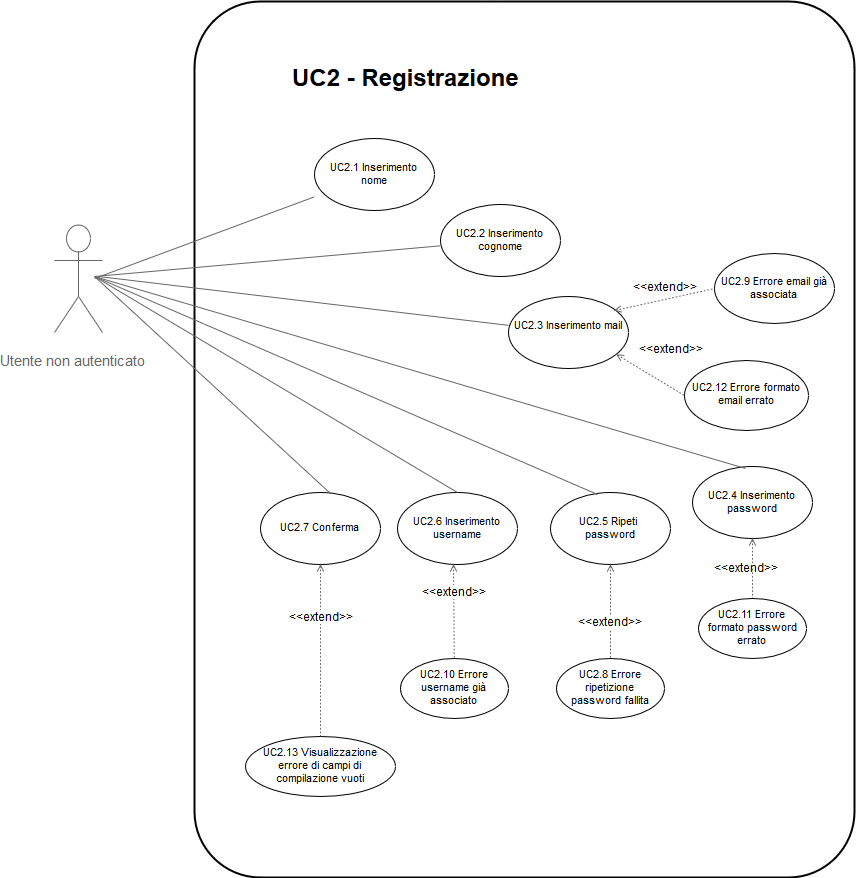
\includegraphics[scale=0.50]{immagini/2.png}
           \caption{Diagramma UC2 - Registrazione}
           \end{center}
        \end{figure}

 
 
        
      \subsubsection{UC 3-Login}
        \begin{itemize}
        \item \textbf{Attori primari}: Utente non autenticato.
        \item \textbf{Attori secondari}: Aws.
        \item \textbf{Scopo e descrizione}: L'utente richiede il login al sistema per accedere al proprio account.
        \item \textbf{Scenario principale}:
            \begin{itemize}
                \item L'utente non autenticato accede alla piattaforma;
                \item L'utente che desidera accedere al proprio account seleziona la funzionalità "Login";
                \item L'utente digita le credenziali di accesso relative al proprio account;
                \item L'utente conferma il login.
            \end{itemize}
         \item \textbf{Scenario secondario}: L'utente non desidera procedere con la conferma del login. Di conseguenza viene mostrata la schermata principale del sistema.
         
        \item \textbf{Precondizione}: L'utente non è riconosciuto nel sistema;
        \item \textbf{Postcondizione}: L'utente viene riconosciuto dal sistema.
        \end{itemize}

   
        \paragraph{UC 3.1-Inserimento username}
            \begin{itemize}
                \item \textbf{Attori primari}: Utente non autenticato;
                
                \item \textbf{Scopo e descrizione}: L'utente inserisce il proprio username per effettuare la login; 
                \item \textbf{Scenario principale}: 
                    \begin{itemize}
                        \item L'utente si trova nella sezione dedicata al login;
                        \item L'utente inserisce il proprio username.
                    \end{itemize}
                \item \textbf{Precondizione}: L'utente si trova in una schermata in cui è possibile inserire il proprio username;
             \item \textbf{Postcondizione}:L'utente ha inserito il proprio username.
           \end{itemize}
        
        \paragraph{UC 3.2-Inserimento password}
            \begin{itemize}
                \item \textbf{Attori primari}: Utente non autenticato;
                
                \item \textbf{Scopo e descrizione}: L'utente inserisce la propria password per effettuare la login. Durante l’inserimento non deve essere possibile leggere la password. Sarà possibile visualizzare
                dei segnaposto per indicare che è stato inserito un carattere della password; 
                \item \textbf{Scenario principale}: 
                    \begin{itemize}
                        \item L'utente si trova nella sezione dedicata al login;
                        \item L'utente inserisce la propria password.
                    \end{itemize}
                \item \textbf{Precondizione}: L'utente si trova in una schermata in cui è possibile inserire la propria password;
             \item \textbf{Postcondizione}:L'utente ha inserito la propria password.
           \end{itemize}
           
        \paragraph{UC 3.3-Conferma login}
            \begin{itemize}
                \item \textbf{Attori primari}: : Utente non autenticato;
                \item \textbf{Scopo e descrizione}: L'utente conferma i dati inseriti precedentemente per effettuare il login; 
                \item \textbf{Scenario principale}:
                    \begin{itemize}
                        \item L'utente si trova nella sezione dedicata al login;
                        \item L'utente conferma l'operazione di login cliccando il pulsante apposito.
                    \end{itemize}
                \item \textbf{Estensioni}: Visualizzazione errore nel caso di autenticazione fallita (UC 3.4), dovuta all'inserimento di credenziali errate;
                \item \textbf{Precondizione}:L'utente si trova in una schermata in cui è possibile dare la conferma dei dati inseriti;
                \item \textbf{Postcondizione}:L’utente ha espresso di voler procedere con la conferma e quindi con il login al sistema.
            \end{itemize}
        
        
        \paragraph{UC 3.4-Autenticazione fallita}
            \begin{itemize}
                \item \textbf{Attori primari}: Utente non autenticato;
                
                \item \textbf{Scopo e descrizione}: La procedura di autenticazione ha riscontrato un errore in merito ai
                dati inseriti durante la procedura di login.  
                   
                \item \textbf{Scenario principale}: 
                    \begin{itemize}
                        \item L'utente ha inserito le proprie credenziali e ha confermato il login;
                        \item Le credenziali inserite dall'utente non sono corrette, pertanto scatenano un errore di autenticazione.
                    \end{itemize}
                \item \textbf{Precondizione}: L'utente ha inserito le proprie credenziali e ha confermato il login;
                 \item \textbf{Postcondizione}: Viene notificato all'utente che si è verificato un errore in merito
                alla procedura di autenticazione. Deve essere indicato specificatamente che tipo di errore si è presentato.
            \end{itemize}
   \newpage
   
   \begin{figure}[h!]
           \begin{center}
           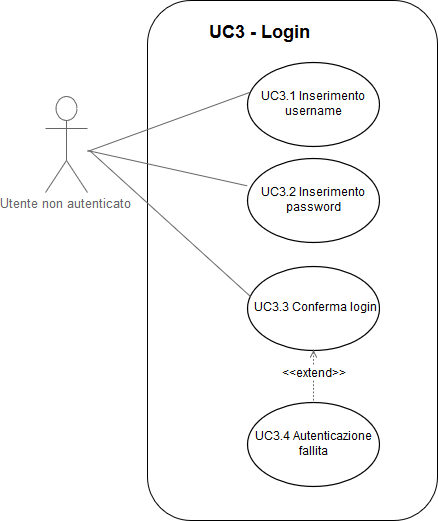
\includegraphics[scale=0.50]{immagini/3.png}
           \caption{Diagramma UC3 - Login}
           \end{center}
  \end{figure}   
          
       
        
     \subsubsection{UC 4-Logout}
        \begin{itemize}
            \item  \textbf{Attori primari}: Utente autenticato;
            \item \textbf{Scopo e descrizione}: L'utente che desidera effettuare il logout clicca su un apposita sezione e dà conferma.
            \item \textbf{Scenario principale}: L'utente precedentemente autenticato richiede il logout dal profilo personale interno all'applicazione;
            \item \textbf{Precondizione}: L'utente è autenticato e il sistema mette a sua disposizione una sezione apposita al logout;
            \item \textbf{Postcondizione}: Il sistema ha elaborato la richiesta di logout dell'utente chiudendo la sua sessione.
        \end{itemize}    
        
        
    \subsubsection{UC 5-Inserimento/modifica dei dati opzionali relativi all'account}  
      \begin{itemize}
        \item \textbf{Attori primari}: Utente autenticato;
        \item \textbf{Attori secondari}: Aws, Facebook;
        \item \textbf{Scopo e descrizione}: L'utente che ha precedentemente creato un profilo inserendo le informazioni obbligatorie desidera arricchire il suo profilo, inserendo per la prima volta o modificando le informazioni esistenti, con informazioni aggiuntive.
        \item \textbf{Scenario principale}:
            \begin{itemize}
                \item L'utente è autenticato con il proprio profilo all'interno del sistema;
                \item L'utente desidera arricchire il profilo inserendo o modificando i dati opzionali a esso associato, pertanto si porta nell'apposita sezione.
            \end{itemize}
        \item \textbf{Scenario secondario}: L'utente non desidera procedere con l'inserimento o la modifica dei dati opzionali;
        \item \textbf{Precondizione}: L'utente autenticato si trova nella propria area personale, nella sezione apposita per l'inserimento o la modifica dei dati opzionali del proprio profilo;
        \item \textbf{Postcondizione}: L'utente ha inserito o modificato i dati opzionali associati al proprio profilo.
        \end{itemize}


        
        \subsubsection{UC 6-Modifica dei dati anagrafici obbligatori del profilo utente}
        \begin{itemize}
        \item \textbf{Attori primari}: Utente autenticato;
        \item \textbf{Attori secondari}: Aws;
        \item \textbf{Scopo e descrizione}: L'utente autenticato è in grado di eseguire operazioni di modifica sui dati personali, precedentemente inseriti in fase di registrazione, o di eliminare il proprio account. I dati modificabili sono quindi:
            \begin{itemize}
                \item Nome;
                \item Cognome;
                \item Username;
                \item E-mail;
                \item Password.
            \end{itemize}
        \item \textbf{Scenario principale}:
            \begin{itemize}
                \item L'utente autenticato accede alla piattaforma;
                \item L'utente che desidera apportare modifiche al proprio account seleziona la specifica sezione per le modifiche all'account;
                \item L'utente modifica i propri dati secondo esigenze;
                \item L'utente conferma le modifiche apportate.
            \end{itemize}
        \item \textbf{Scenario secondario}: L'utente interrompe l'inserimento delle modifiche sui dati e le modifiche non vengono memorizzate dal sistema.
         \textbf{Precondizione}: L'utente autenticato ha scelto di apportare modifiche al proprio account;
        \item \textbf{Postcondizione}: Il sistema ha memorizzato le modifiche desiderate e permesse che l’utente ha apportato al proprio profilo.
        \end{itemize}
        
         \paragraph{UC 6.1-Modifica password}
            \begin{itemize}
                \item \textbf{Attori primari}: Utente autenticato;
               
                \item \textbf{Scopo e descrizione}: L'utente desidera modificare la propria password; 
                \item \textbf{Scenario principale}:
                    \begin{itemize}
                        \item L'utente si trova nella sezione dedicata alla modifica dei dati relativi all'account utente;
                        \item L'utente modifica la password relativa all'account.
                    \end{itemize}
                \item \textbf{Scenario secondario}: L'utente non desidera continuare con la modifica della password e termina l'inserimento. Il sistema non memorizza le modifiche apportate;
                 \item \textbf{Inclusioni}: 
                    \begin{itemize}
                        \item L'utente per poter memorizzare la nuova password deve inserire la password precedente (UC 6.1.1);
                        \item  L'utente per poter memorizzare la nuova password deve ripetere la password all'interno del campo "Ripeti password" (UC 2.5);
                    \end{itemize}
                \item \textbf{Estensioni}:
                    \begin{itemize}
                        \item La nuova password inserita è uguale a quella precedente (UC 6.1.2);
                        \item La conferma della nuova password inserita non coincide con la prima digitata (UC 2.8);
                        \item Il formato della nuova password inserita non è corretto (UC 2.11).
                    \end{itemize}
               
                \item \textbf{Precondizione}: L'utente si trova in una schermata in cui è possibile modificare la password associata al proprio profilo;
                \item \textbf{Postcondizione}:L’utente ha espresso di voler procedere con la conferma e quindi
                con la modifica della password associata al suo profilo.
            \end{itemize}
        
            \subparagraph{UC 6.1.1-Inserisci vecchia password}
                \begin{itemize}
                \item \textbf{Attori primari}: Utente autenticato;
               
                \item \textbf{Scopo e descrizione}: L'utente deve inserire la vecchia password per poterne inserire una nuova;
                \item \textbf{Scenario principale}:
                    \begin{itemize}
                        \item L'utente si trova nella sezione dedicata alla modifica dei dati personali relativi all'account utente;
                        \item L'utente inserisce la password antecedente relativa all'account per poterla aggiornare.
                    \end{itemize}
                \item \textbf{Precondizione}: L'utente si trova in una schermata in cui è possibile modificare i dati utente relativi all'account, nello specifico la password associata all'account;
                \item \textbf{Postcondizione}: L’utente ha inserito la vecchia password correttamente al fine di aggiornarla.
            \end{itemize}
        
        
         \subparagraph{UC 6.1.2-La nuova password coincide con quella precedente}
             \begin{itemize}
                \item \textbf{Attori primari}: Utente autenticato;
               
                \item \textbf{Scopo e descrizione}: L'utente deve inserire la vecchia password per poterne inserire una nuova, ma si verifica un errore dal momento che la nuova password inserita coincide con quella precedente.
                \item \textbf{Scenario principale}:
                    \begin{itemize}
                        \item L'utente si trova nella sezione dedicata alla modifica dei dati personali relativi all'account utente, nello specifico sta modificando la password associata al proprio account;
                        \item L'utente inserisce una nuova password uguale a quella precedente.
                    \end{itemize}
                \item \textbf{Precondizione}: L'utente si trova in una schermata in cui è possibile modificare i dati utente relativi all'account, nello specifico la password associata all'account;
                \item \textbf{Postcondizione}:L’utente non ha modificato la propria password poiché ha inserito una nuova password che coincide con quella vecchia: il sistema non registra le modifiche.
            \end{itemize}
        
        
        \paragraph{UC 6.2-Modifica mail}
            \begin{itemize}
                \item \textbf{Attori primari}: Utente autenticato;
               
                \item \textbf{Scopo e descrizione}: L'utente desidera modificare la mail associata all'account; 
                \item \textbf{Scenario principale}:
                    \begin{itemize}
                        \item L'utente si trova nella sezione dedicata alla modifica dei dati relativi all'account utente;
                        \item L'utente modifica la mail relativa all'account.
                    \end{itemize}
                \item \textbf{Estensioni}:
                    \begin{itemize}
                        \item La nuova mail è già associata a un profilo esistente (UC 2.9).
                        \item Il formato della nuova mail non è valido(UC 2.12).
                      \end{itemize}
                \item \textbf{Precondizione}: L'utente si trova in una schermata in cui è possibile modificare la propria mail;
                \item \textbf{Postcondizione}:L’utente ha espresso di voler procedere con la conferma e quindi
                con la modifica della propria mail.
            \end{itemize}
        
        \paragraph{UC 6.3-Modifica Nome}
            \begin{itemize}
                \item \textbf{Attori primari}: Utente autenticato;
                
                \item \textbf{Scopo e descrizione}: L'utente desidera modificare il nome associato al proprio account; 
                \item \textbf{Scenario principale}:
                    \begin{itemize}
                        \item L'utente si trova nella sezione dedicata alla modifica dei dati relativi al proprio account;
                        \item L'utente modifica il nome relativo all'account.
                    \end{itemize}
                \item \textbf{Precondizione}: L'utente si trova in una schermata in cui è possibile modificare il proprio nome;
                \item \textbf{Postcondizione}:L’utente ha espresso di voler procedere con la conferma e quindi
                con la modifica del proprio nome.
            \end{itemize}
            
            
        \paragraph{UC 6.4-Modifica cognome}
            \begin{itemize}
                \item \textbf{Attori primari}: Utente autenticato;
                
                \item \textbf{Scopo e descrizione}: L'utente desidera modificare il cognome associato al proprio account; 
                \item \textbf{Scenario principale}:
                    \begin{itemize}
                        \item L'utente si trova nella sezione dedicata alla modifica dei dati relativi all'account utente;
                        \item L'utente modifica il cognome relativo all'account.
                    \end{itemize}
               
                \item \textbf{Precondizione}: L'utente si trova in una schermata in cui è possibile modificare il proprio cognome;
                \item \textbf{Postcondizione}:L’utente ha espresso di voler procedere con la conferma e quindi
                con la modifica del proprio cognome.
            \end{itemize}
            
         \paragraph{UC 6.5-Eliminazione account}
            \begin{itemize}
                \item \textbf{Attori primari}: Utente autenticato;
                
                \item \textbf{Scopo e descrizione}: L'utente in possesso di un account desidera cancellare il proprio profilo dalla piattaforma; 
                \item \textbf{Scenario principale}:
                    \begin{itemize}
                        \item L'utente si trova nella sezione dedicata alla cancellazione del profilo;
                        \item L'utente conferma la cancellazione del profilo.
                    \end{itemize}
               
                \item \textbf{Precondizione}: L'utente si trova in una schermata in cui è possibile cancellare il profilo;
                \item \textbf{Postcondizione}:L’utente ha espresso di voler procedere con la cancellazione e quindi
                il sistema ne cancella il profilo e i relativi dati.
            \end{itemize}
            
            
        \paragraph{UC 6.6-Conferma modifiche}
            \begin{itemize}
                \item \textbf{Attori primari}: Utente autenticato;
                
                \item \textbf{Scopo e descrizione}: L'utente conferma le modifiche inserite precedentemente per        permettere al sistema di memorizzarle; 
                \item \textbf{Scenario principale}:
                    \begin{itemize}
                        \item L'utente si trova nella sezione dedicata alla modifica dei dati relativi all'account utente;
                        \item L'utente conferma l'operazione di modifica cliccando il pulsante apposito.
                    \end{itemize}
                    \item \textbf{Estensioni}: La registrazione può fallire a causa del seguente errore di compilazione da parte dell'utente:
                    \begin{itemize}
                    \item Esistono dei campi vuoti (UC 2.13).
                    \end{itemize}
                \item \textbf{Precondizione}: L'utente si trova in una schermata in cui è possibile dare la conferma
                dell'operazione di modifica;
                \item \textbf{Postcondizione}: L’utente ha espresso di voler procedere con la conferma e quindi
                con la memorizzazione dei nuovi dati.
            \end{itemize}
        
   \begin{figure}[h!]
           \begin{center}
           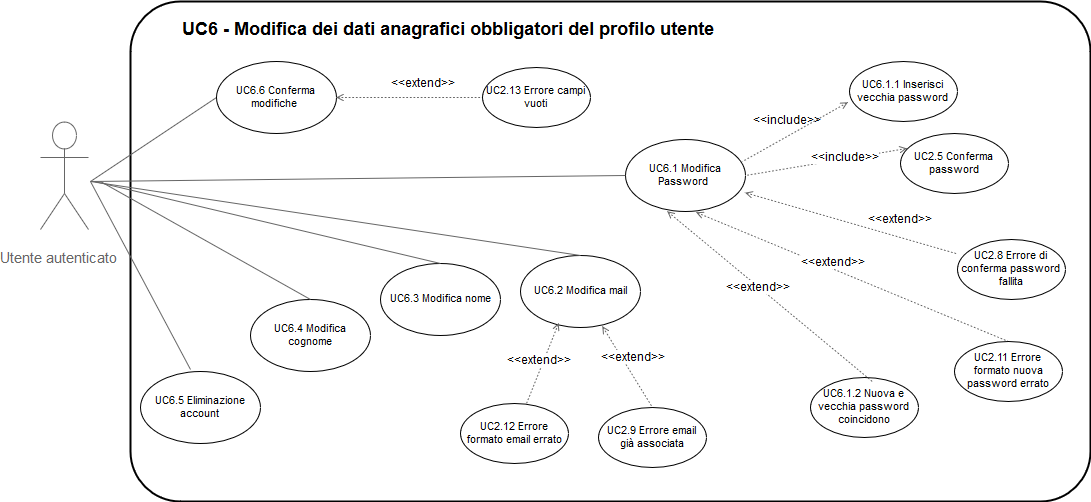
\includegraphics[scale=0.38]{immagini/6.png}
           \caption{Diagramma UC6 - Modifica dei dati anagrafici obbligatori del profilo utente}
           \end{center}
   \end{figure}
     
        
        
    \subsubsection{UC 7-Gestione dati delle macchine utente}
      \begin{itemize}
                \item \textbf{Attori primari}: Utente autenticato;
                \item \textbf{Attori secondari}: Aws;
                 \item \textbf{Scopo e descrizione}: L'utente è in grado di eseguire operazioni di inserimento, modifica e rimozione sulle auto associate al proprio profilo, ovvero le auto che l'utente rende disponibili sulla piattaforma ad altre persone all'interno del sistema per consentire loro di effettuare un viaggio;
                 \item \textbf{Scenario principale}: 
                 \begin{itemize}
                     \item L'utente autenticato accede alla piattaforma;
                     \item L’utente che desidera inserire, rimuovere o modificare auto dal proprio account seleziona la specifica sezione per la gestione delle auto;
                     \item L'utente apporta modifiche secondo le proprie esigenze;
                 \end{itemize}
                 \item \textbf{Scenario secondario} L'utente non desidera continuare l'operazione di inserimento/modifica/eliminazione dell'auto, interrompe il processo e le modifiche non vengono memorizzate dal sistema;
                 \item \textbf{Precondizione}: L'utente autenticato ha scelto di inserire, modificare o rimuovere una vettura all'interno del proprio profilo;
                 \item \textbf{Postcondizione}: Il sistema ha memorizzato le modifiche desiderate e permesse che l'utente ha apportato alla sezione auto.
                 \end{itemize}

       
     \begin{figure}[h!]
           \begin{center}
           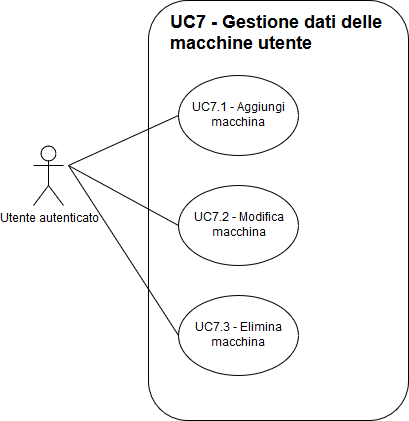
\includegraphics[scale=0.50]{immagini/7.png} 
           \caption{Diagramma UC7 - Gestione dati delle macchine utente}
           \end{center}
        \end{figure}
        
        \newpage
                 
                 \paragraph{UC 7.1-Aggiungi macchina}
                 \begin{itemize}
                \item \textbf{Attori primari}: Utente autenticato;
                
                 \item \textbf{Scopo e descrizione}: L'utente desidera aggiungere un'auto da mettere a disposizione all'interno della piattaforma;
                 \item \textbf{Scenario principale}: L'utente si trova nella sezione di gestione dati della macchina utente e richiede al sistema di inserire un'auto da mettere a disposizione;
                 \item \textbf{Scenario secondario}: L'utente interrompe l'inserimento dei dati e l'aggiunta non viene memorizzata dal sistema.
                
                
                 \item \textbf{Precondizione}: L'utente vuole aggiungere un auto da mettere a disposizione all'interno del sistema;
                 \item \textbf{Postcondizione}: L'utente ha inserito l'auto all'interno del sistema.
                 \end{itemize}
                 
    \subparagraph{UC 7.1.1-Inserimento targa}
    \begin{itemize}
                \item \textbf{Attori primari}: Utente autenticato;
                
                 \item \textbf{Scopo e descrizione}: L'utente compila il campo targa per effettuare la registrazione della propria auto;
                 \item \textbf{Scenario principale}: L'utente si trova nella sezione aggiungi auto e richiede al sistema di inserire la targa della propria macchina;
                 \item \textbf{Estensioni}: 
                 \begin{itemize}
                 \item Il formato della targa inserita non è valido(7.1.12);
                 \item La targa é già associata ad un'altra macchina presente nel sistema(7.1.13).
                 \end{itemize}
                 \item \textbf{Precondizione}: Il sistema fornisce una schermata in cui è possibile inserire la targa della propria auto;
                 \item \textbf{Postcondizione}:L’utente ha compilato il campo "Targa".
                 \end{itemize}
                 
    
                 
    \subparagraph{UC 7.1.2-Inserimento marca}
    \begin{itemize}
                \item \textbf{Attori primari}: Utente autenticato;
                
                 \item \textbf{Scenario principale}: L'utente compila il campo marca per effettuare la registrazione della propria auto;
                 \item \textbf{Scopo e descrizione}: 
                 \begin{itemize}
                     \item L'utente si trova nell'apposita sezione di gestione dati della macchina;
                     \item L'utente compila il campo "Marca".
                 \end{itemize}
                 \item \textbf{Precondizione}: Il sistema fornisce una schermata in cui è possibile inserire la marca dell'auto;
                 \item \textbf{Postcondizione}: L'utente ha compilato il campo "Marca".
                 \end{itemize}
                 
    \subparagraph{UC 7.1.3-Inserimento modello}
    \begin{itemize}
                \item \textbf{Attori primari}: Utente autenticato;
                
                 \item \textbf{Scopo e descrizione}: L'utente compila il campo modello per effettuare la registrazione della propria auto;
                 \item \textbf{Scenario principale}:
                 \begin{itemize}
                     \item L'utente si trova nell'apposita sezione di gestione dati della macchina;
                     \item L'utente compila il campo "Modello".
                 \end{itemize}
                 \item \textbf{Precondizione}: Il sistema fornisce una schermata in cui è possibile inserire il modello dell'auto;
                 \item \textbf{Postcondizione}: L'utente ha compilato il campo "Modello".
                 \end{itemize}
                 
   \subparagraph{UC 7.1.4-Inserimento anno di produzione}
   \begin{itemize}
                \item \textbf{Attori primari}: Utente autenticato;
                
                 \item \textbf{Scopo e descrizione}: L'utente compila il campo anno di produzione per effettuare la registrazione della propria auto;
                 \item \textbf{Scenario principale}: 
                 \begin{itemize}
                     \item L'utente si trova nell'apposita sezione di gestione dati della macchina;
                     \item L'utente compila il campo "Anno di produzione".
                 \end{itemize}
                 \item \textbf{Estensioni}:
                    \begin{itemize}
                        \item L'utente tenta di inserire un formato per l'anno di produzione errato, ovvero minore di zero (UC 7.1.14).
                    \end{itemize}
                 \item \textbf{Precondizione}: Il sistema fornisce una schermata in cui è possibile inserire l'anno di produzione dell'auto;
                 \item \textbf{Postcondizione}: L'utente ha compilato il campo "Anno di produzione".
                 \end{itemize}
                 
    \subparagraph{UC 7.1.5-Inserimento cavalli motore}
    \begin{itemize}
                \item \textbf{Attori primari}: Utente autenticato;
                
                 \item \textbf{Scopo e descrizione}: L'utente compila il campo  cavalli motore per effettuare la registrazione della propria auto;
                 \item \textbf{Scenario principale}: 
                 \begin{itemize}
                     \item L'utente si trova nell'apposita sezione di gestione dati della macchina;
                     \item L'utente compila il campo "Cavalli motore".
                 \end{itemize}
                 \item \textbf{Estensioni}:
                 \begin{itemize} 
                        \item L'utente tenta di inserire un formato per il numero di cavalli motore errato, ovvero minore di zero (UC 7.1.14).
                    \end{itemize}
                 \item \textbf{Precondizione}: Il sistema fornisce una schermata in cui è possibile inserire i cavalli dell'auto;
                 \item \textbf{Postcondizione}: L'utente ha compilato il campo "Cavalli motore".
                 \end{itemize}
                 
                 \subparagraph{UC 7.1.6-Inserimento cilindrata motore}
    \begin{itemize}
                \item \textbf{Attori primari}: Utente autenticato;
               
                 \item \textbf{Scopo e descrizione}: L'utente compila il campo cilindrata motore per effettuare la registrazione della propria auto;
                 \item \textbf{Scenario principale}: 
                 \begin{itemize}
                     \item L'utente si trova nell'apposita sezione di gestione dati della macchina;
                     \item L'utente compila il campo "Cilindrata motore".
                 \end{itemize}
                 \item \textbf{Estensioni}:
                 \begin{itemize}
                        \item L'utente tenta di inserire un formato per la cilindrata del motore errato, ovvero minore di zero (UC 7.1.14).
                    \end{itemize}
                 \item \textbf{Precondizione}: Il sistema fornisce una schermata in cui è possibile inserire la cilindrata dell'auto;
                 \item \textbf{Postcondizione}: L'utente ha compilato il campo "Cilindrata motore".
                 \end{itemize}
                 
                 \subparagraph{UC 7.1.7-Inserimento raggio di percorrenza consentito}
    \begin{itemize}
                \item \textbf{Attori primari}: Utente autenticato;
                
                 \item \textbf{Scopo e descrizione}: L'utente compila il campo raggio motore per effettuare la registrazione della propria auto;
                 \item \textbf{Scenario principale}:
                 \begin{itemize}
                     \item L'utente si trova nell'apposita sezione di gestione dati della macchina;
                     \item L'utente compila il campo "Raggio".
                 \end{itemize}
                 \item \textbf{Estensioni}:
                 \begin{itemize}
                        \item L'utente tenta di inserire un formato per il raggio di produzione consentito errato, ovvero minore di zero (UC 7.1.14).
                    \end{itemize}
                 \item \textbf{Precondizione}: Il sistema fornisce una schermata in cui è possibile inserire il raggio dell'auto;
                 \item \textbf{Postcondizione}: L'utente ha compilato il campo "Raggio".
                 \end{itemize}
                 
        \subparagraph{UC 7.1.8-Inserimento chilometraggio}
    \begin{itemize}
                \item \textbf{Attori primari}: Utente autenticato;
               
                 \item \textbf{Scopo e descrizione}: L'utente compila il campo chilometraggio della macchina per effettuarne la registrazione;
                 \item \textbf{Scenario principale}: L'utente si trova nella sezione aggiungi auto e richiede al sistema di inserire il chilometraggio effettuato dalla propria macchina;
                 \item \textbf{Estensioni}: 
                 \begin{itemize}
                        \item L'utente tenta di inserire un formato per il numero di chilometri effettuati dalla macchina errato, ovvero minore di zero (UC 7.1.14).
                    \end{itemize}
                 \item \textbf{Precondizione}: L'utente desidera inserire il chilometraggio della propria auto;
                 \item \textbf{Postcondizione}:L’utente ha compilato il campo "Chilometri percorsi dall'auto".
                 \end{itemize}
                 
        \subparagraph{UC 7.1.9-Inserimento calendario disponibilità}
    \begin{itemize}
                \item \textbf{Attori primari}: Utente autenticato;
              
                 \item \textbf{Scopo e descrizione}: L'utente compila il campo calendario disponibilità per effettuare la registrazione della propria auto;
                 \item \textbf{Scenario principale}: L'utente si trova nella sezione aggiungi auto e richiede al sistema di inserire il calendario relativo alla propria macchina;
                 
                 \item \textbf{Precondizione}: L'utente desidera inserire il calendario di disponibilità della propria auto;
                 \item \textbf{Postcondizione}:L’utente ha compilato il campo "Calendario disponibilità".
                 \end{itemize}
                 
                 
            \subparagraph{UC 7.1.10-Inserimento tariffa oraria}
    \begin{itemize}
                \item \textbf{Attori primari}: Utente autenticato;
               
                 \item \textbf{Scopo e descrizione}: L'utente compila il campo tariffa oraria per effettuare la registrazione della propria auto;
                 \item \textbf{Scenario principale}: L'utente si trova nella sezione aggiungi auto e richiede al sistema di inserire la tariffa oraria relativa alla propria macchina;
                 \item \textbf{Estensioni}:
                    \begin{itemize}
                        \item L'utente tenta di inserire un formato per la tariffa oraria errato, ovvero minore di zero (UC 7.1.14).
                    \end{itemize}
                 \item \textbf{Precondizione}: L'utente desidera inserire la tariffa oraria della propria auto;
                 \item \textbf{Postcondizione}:L’utente compila il campo "Tariffa oraria".
                 \end{itemize}
                 
                 
                 
            \subparagraph{UC 7.1.11-Visualizzazione messaggio errore campi di compilazione vuoti}
    \begin{itemize}
                \item \textbf{Attori primari}: Utente autenticato;
               
                 \item \textbf{Scopo e descrizione}: La procedura di registrazione ha riscontrato un errore in merito ai
                dati inseriti. Nello specifico l'errore è dovuto al fatto che esiste almeno un campo di compilazione lasciato vuoto.
                 \item \textbf{Scenario principale}: 
                 \begin{itemize}
                     \item L'utente ha inserito i dati per la registrazione della macchina;
                     \item L'utente non ha compilato uno o più campi.
                 \end{itemize}
                 \item \textbf{Precondizione}: L'utente ha inserito i dati della sua auto e ha confermato la registrazione. L'utente tenta di aggiungere la propria auto non compilando tutti i campi.
                 \item \textbf{Postcondizione}: Viene notificato all'utente che si è verificato un errore in merito alla procedura di aggiungere un auto. L'utente ora è consapevole del fatto che deve compilare tutti i campi per aggiungere un auto.
                 \end{itemize}
                 
                 
                \subparagraph{UC 7.1.12-Visualizzazione messaggio errore formato targa non valido} 
    \begin{itemize}
                \item \textbf{Attori primari}: Utente autenticato;
               
                 \item \textbf{Scopo e descrizione}: La procedura di inserimento della targa ha riscontrato un errore perché il formato non è valido, quindi:
                
              
                 \item \textbf{Scenario principale}: 
                 \begin{itemize}
                     \item L'utente ha inserito la targa;
                     \item Il formato della targa inserita nel campo "Targa" non è corretto, pertanto viene scatenato un errore.
                 \end{itemize}
                 \item \textbf{Precondizione}:  L'utente tenta di aggiungere un auto avente il formato della targa errato.
                 \item \textbf{Postcondizione}: Viene notificato all'utente che si è verificato un errore in merito alla registrazione dell'auto. L'utente ora è consapevole del fatto che il formato della targa inserita non è consentito.
                 \end{itemize}
                 
                 \subparagraph{UC 7.1.13-Visualizzazione messaggio errore targa già esistente}
    \begin{itemize}
                \item \textbf{Attori primari}: Utente autenticato;
               
                 \item \textbf{Scopo e descrizione}: La procedura di registrazione dell'auto ha riscontrato un errore in merito ai dati inseriti. Nello specifico l'errore è dovuto al fatto che la targa inserita nel campo "Targa" è già associata a un'altra macchina presente nella piattaforma.
                 \item \textbf{Scenario principale}:
                 \begin{itemize}
                     \item L'utente ha inserito i dati della propria macchina per metterla a disposizione;
                     \item La targa inserita nel campo "Targa" è associata a un'altra macchina,pertanto viene scatenato un errore.
                 \end{itemize}
                 \item \textbf{Precondizione}: L'utente ha inserito tutti i dati per la registrazione dell'auto. L'utente tenta di registrare la macchina usando una targa già esistente.
                 \item \textbf{Postcondizione}: Viene notificato all'utente che si è verificato un errore in merito alla procedura di registrazione. L’utente ora è consapevole del fatto che la targa inserita è già associata ad un'altra macchina.
                 \end{itemize}
                 
                 
                 \subparagraph{UC 7.1.14-Visualizzazione messaggio errore campo minore di zero} 
    \begin{itemize}
                \item \textbf{Attori primari}: Utente autenticato;
               
                 \item \textbf{Scopo e descrizione}: Durante la procedura di inserimento dei dati si è sollevata una condizione di errore. Nel particolare l'errore si può riscontrare in uno dei seguenti campi: anno di produzione, cavalli motore, cilindrata del motore, raggio di percorrenza consentito o chilometri effettuati dall'auto. La procedura di inserimento ha riscontrato un errore perché il formato inserito in almeno uno dei campi non è valido, ovvero si inserisce un numero minore di zero.
                 \item \textbf{Scenario principale}: 
                 \begin{itemize}
                     \item L'utente ha inserito i dati di anno di produzione, cavalli motore, cilindrata del motore, raggio di percorrenza consentito e chilometri fatti;
                     \item Il formato di almeno uno di questi campi è minore di zero, quindi non corretto. Viene scatenato un errore.
                 \end{itemize}
                 \item \textbf{Precondizione}: L'utente ha inserito i dati della macchina per poterla mettere a disposizione. L'utente tenta di aggiungere un auto avente il formato di almeno uno dei campi sopracitati errato.
                 \item \textbf{Postcondizione}: Viene notificato all'utente che si è verificato un errore in merito all'aggiunta dell'auto. L'utente ora è consapevole del fatto che il formato di almeno uno dei campi sopracitati non è consentito.
                 \end{itemize}
         
         \subparagraph{UC 7.1.15-Conferma aggiunta dell'auto}
            \begin{itemize}
                \item \textbf{Attori primari}: Utente autenticato;
                
                \item \textbf{Scopo e descrizione}: L'utente conferma l' operazione di aggiunta dell'auto al proprio profilo; 
                \item \textbf{Scenario principale}:
                    \begin{itemize}
                        \item L'utente si trova nella sezione dedicata all'aggiunta di un'auto all'interno del proprio profilo;
                        \item L'utente conferma l'operazione di aggiunta cliccando il pulsante apposito.
                    \end{itemize}
                \item \textbf{Estensioni}: La registrazione può fallire a causa del seguente errore di compilazione da parte dell'utente:
                \begin{itemize}
                \item Esistono dei campi vuoti (UC 7.1.11).
                \end{itemize}
                \item \textbf{Precondizione}: L'utente si trova in una schermata in cui è possibile dare la conferma
                dei dati inseriti per l'aggiunta dell'auto all'interno del proprio profilo;
                \item \textbf{Postcondizione}:L’utente ha espresso di voler procedere con la conferma dell'operazione e quindi il sistema memorizza la decisione.
            \end{itemize}
                        
                 
                 
           \begin{figure}[h!]
           \begin{center}
           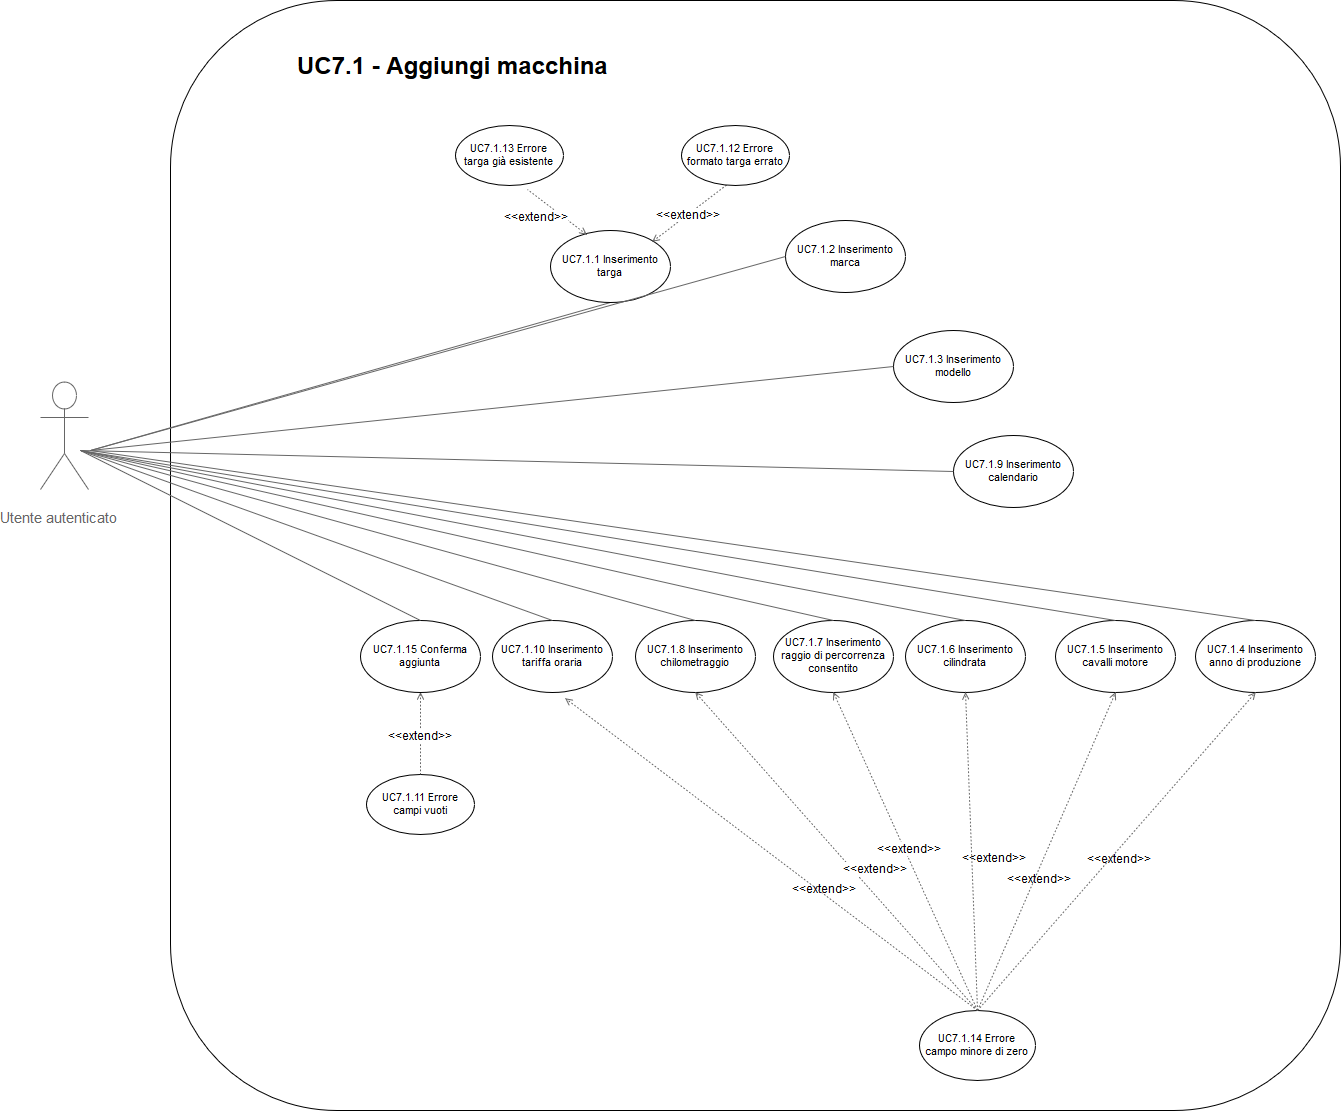
\includegraphics[scale=0.3]{immagini/71.png}   
           \caption{Diagramma UC7.1 - Aggiungi macchina}
           \end{center}
           \end{figure}      
           
           \newpage      
                       
                     
    \paragraph{UC 7.2-Modifica macchina}
    \begin{itemize}
                \item \textbf{Attori primari}: Utente autenticato;
                
                 \item \textbf{Scopo e descrizione}: L'utente desidera modificare un'auto all'interno del proprio profilo da mettere a disposizione;
                 \item \textbf{Scenario principale}:
                 \begin{itemize}
                    \item L'utente autenticato accede alla piattaforma;
                    \item L'utente che desidera apportare modifiche al proprio veicolo seleziona la specifica sezione indicante il proprio parco macchine;
                    \item L'utente seleziona l'auto da modificare;
                    \item L'utente modifica i propri dati secondo esigenze;
                    \item L'utente conferma le modifiche apportate.
                \end{itemize}
                \item \textbf{Scenario secondario}: L'utente interrompe l'inserimento delle modifiche sui dati e le modifiche non vengono memorizzate dal sistema.
                
                 \item \textbf{Precondizione}: L'utente ha già inserito almeno un auto all'interno del proprio profilo e vuole modificare una delle macchine da mettere a disposizione all'interno del sistema;
                 \item \textbf{Postcondizione}: L'utente ha modificato l'auto all'interno del sistema.
                 \end{itemize}
    
    \subparagraph{UC 7.2.1-Selezione macchina da modificare}
    \begin{itemize}
                \item \textbf{Attori primari}: Utente autenticato;
               
                 \item \textbf{Scopo e descrizione}: L’utente seleziona l'auto (tra quelle da lui precedentemente inserite all'interno del proprio account) sulla quale vuole effettuare l'operazione di modifica dei dati;
                 \item \textbf{Scenario principale}: 
                 \begin{itemize}
                     \item L’utente si trova nella sezione dedicata alla modifica dei dati relativi alle macchine dell'utente;
                     \item L'utente seleziona una delle macchine associate al suo account sulla quale vuole eseguire l'operazione di modifica.          \end{itemize}
                 \item \textbf{Precondizione}: L’utente si trova in una schermata in cui selezionare su quale macchina è possibile effettuare l'operazione di modifica;
                 \item \textbf{Postcondizione}: L’utente seleziona l'auto sulla quale vuole effettuare la modifica dei relativi dati (targa, marca, modello, anno di produzione, cavalli motore, cilindrata, raggio consentito, kilometraggio, calendario disponibilità o tariffa oraria).
                 \end{itemize}
    
    \subparagraph{UC 7.2.2-Conferma modifica}
    \begin{itemize}
                \item \textbf{Attori primari}: Utente autenticato;;
                
                 \item \textbf{Scopo e descrizione}: L’utente conferma le modifiche inserite precedentemente per permettere al sistema di memorizzarle;
                 \item \textbf{Scenario principale}: 
                 \begin{itemize}
                     \item L’utente si trova nella sezione dedicata alla modifica dei dati relativi alle macchine dell'utente;
                     \item L'utente conferma l'operazione di modifica cliccando il pulsante apposito. 
                 \end{itemize}
                 \item \textbf{Estensioni}:
            \begin{itemize}
                \item Le modifiche non vengono salvate nel caso l'utente lasci dei campi di compilazione vuoti (UC 7.1.11).
            \end{itemize}
                 \item \textbf{Precondizione}: L’utente si trova in una schermata in cui è possibile dare la conferma dell'operazione di modifica;
                 \item \textbf{Postcondizione}: L’utente ha espresso di voler procedere con la conferma e quindi con la modifica ai propri dati.
                 \end{itemize}
                 
    \subparagraph{UC 7.2.3-Modifica targa}
            \begin{itemize}
                \item \textbf{Attori primari}: Utente autenticato;
                
                \item \textbf{Scopo e descrizione}: L'utente seleziona una delle auto associate al proprio account e ne modifica il numero di targa; 
                \item \textbf{Scenario principale}:
                    \begin{itemize}
                        \item L'utente si trova nella sezione dedicata alla modifica dei dati relativi alle macchine precedentemente inserite dall'utente nel suo account personale;
                        \item L'utente autenticato ha selezionato una delle auto da lui messe a disposizione sulla quale desidera effettuare l'operazione di modifica;
                        \item L'utente modifica la targa relativa a una determinata macchina dell'account.
                    \end{itemize}
                \item \textbf{Scenario secondario}: L'utente non desidera continuare con l'operazione di modifica. Le modifiche pertanto non vengono salvate;
                \item \textbf{Estensioni}:
                    \begin{itemize}
                        \item La nuova targa inserita non è nel formato corretto (UC 7.1.12);
                        \item La nuova targa inserita è già associata ad un'altra macchina presente nel sistema (UC 7.1.13).
                    \end{itemize}
                \item \textbf{Precondizione}: L'utente si trova in una schermata in cui è possibile modificare i dati relativi alla targa di una delle auto associate all'account, precedentemente selezionata;
                \item \textbf{Postcondizione}:L'utente modifica il numero di targa associato a una delle macchine del suo account.
            \end{itemize}
    
    
    \subparagraph{UC 7.2.4-Modifica marca}
            \begin{itemize}
                \item \textbf{Attori primari}: Utente autenticato;
               
                \item \textbf{Scopo e descrizione}: L'utente seleziona una delle auto associate al proprio account e ne modifica la marca; 
                \item \textbf{Scenario principale}:
                    \begin{itemize}
                        \item L'utente si trova nella sezione dedicata alla modifica dei dati relativi alle macchine precedentemente inserite dall'utente nel suo account personale;
                        \item L'utente autenticato ha selezionato una delle auto da lui messe a disposizione sulla quale desidera effettuare l'operazione di modifica;
                        \item L'utente modifica la marca relativa a una determinata macchina dell'account.
                    \end{itemize}
                \item \textbf{Scenario secondario}: L'utente non desidera continuare con l'operazione di modifica. Le modifiche pertanto non vengono salvate;
        
                \item \textbf{Precondizione}: L'utente si trova in una schermata in cui è possibile modificare i dati relativi alla marca di una delle auto associate all'account, precedentemente selezionata;
                \item \textbf{Postcondizione}:L'utente modifica la marca associata a una delle macchine del suo account.
            \end{itemize}
    
    \subparagraph{UC 7.2.5-Modifica modello}
            \begin{itemize}
                \item \textbf{Attori primari}: Utente autenticato;
               
                \item \textbf{Scopo e descrizione}: L'utente seleziona una delle auto associate al proprio account e ne modifica il modello; 
                \item \textbf{Scenario principale}:
                    \begin{itemize}
                        \item L'utente si trova nella sezione dedicata alla modifica dei dati relativi alle macchine precedentemente inserite dall'utente nel suo account personale;
                        \item L'utente autenticato ha selezionato una delle auto da lui messe a disposizione sulla quale desidera effettuare l'operazione di modifica;
                        \item L'utente modifica il modello relativo a una determinata macchina dell'account.
                    \end{itemize}
                \item \textbf{Scenario secondario}: L'utente non desidera continuare con l'operazione di modifica. Le modifiche pertanto non vengono salvate;
        
                \item \textbf{Precondizione}: L'utente si trova in una schermata in cui è possibile modificare i dati relativi al modello di una delle auto associate all'account, precedentemente selezionata;
                \item \textbf{Postcondizione}:L'utente modifica il modello associata a una delle macchine del suo account.
            \end{itemize}
            
            
            \subparagraph{UC 7.2.6-Modifica anno di produzione}
            \begin{itemize}
                \item \textbf{Attori primari}: Utente autenticato;
                
                \item \textbf{Scopo e descrizione}: L'utente seleziona una delle auto associate al proprio account e ne modifica l'anno di produzione; 
                \item \textbf{Scenario principale}:
                    \begin{itemize}
                        \item L'utente si trova nella sezione dedicata alla modifica dei dati relativi alle macchine precedentemente inserite dall'utente nel suo account personale;
                        \item L'utente autenticato ha selezionato una delle auto da lui messe a disposizione sulla quale desidera effettuare l'operazione di modifica;
                        \item L'utente modifica l'anno di produzione relativo a una determinata macchina dell'account.
                    \end{itemize}
                \item \textbf{Scenario secondario}: L'utente non desidera continuare con l'operazione di modifica. Le modifiche pertanto non vengono salvate;
                \item \textbf{Estensioni}:
                    \begin{itemize}
                        \item Viene sollevato un errore nel caso l'utente tenti di aggiornare l'anno di produzione dell'auto in un formato non corretto, ovvero minore di zero (UC 7.1.14); 
                    \end{itemize}
                \item \textbf{Precondizione}: L'utente si trova in una schermata in cui è possibile modificare i dati relativi all'anno di produzione di una delle auto associate all'account, precedentemente selezionata;
                \item \textbf{Postcondizione}:L'utente modifica l'anno di produzione associato a una delle macchine del suo account.
            \end{itemize}
            
            
            \subparagraph{UC 7.2.7-Modifica cavalli motore}
            \begin{itemize}
                \item \textbf{Attori primari}: Utente autenticato;
              
                \item \textbf{Scopo e descrizione}: L'utente seleziona una delle auto associate al proprio account e ne modifica i cavalli motore; 
                \item \textbf{Scenario principale}:
                    \begin{itemize}
                        \item L'utente si trova nella sezione dedicata alla modifica dei dati relativi alle macchine precedentemente inserite dall'utente nel suo account personale;
                        \item L'utente autenticato ha selezionato una delle auto da lui messe a disposizione sulla quale desidera effettuare l'operazione di modifica;
                        \item L'utente modifica i cavalli motore relativi a una determinata macchina dell'account.
                    \end{itemize}
                \item \textbf{Scenario secondario}: L'utente non desidera continuare con l'operazione di modifica. Le modifiche pertanto non vengono salvate;
                \item \textbf{Estensioni}:
                    \begin{itemize}
                        \item Viene sollevato un errore nel caso l'utente tenti di aggiornare il numero di cavalli motore dell'auto in un formato non corretto, ovvero minore di zero (UC 7.1.14); 
                    \end{itemize}
                \item \textbf{Precondizione}: L'utente si trova in una schermata in cui è possibile modificare i dati relativi ai cavalli motore di una delle auto associate all'account, precedentemente selezionata;
                \item \textbf{Postcondizione}:L'utente modifica i cavalli motore associati a una delle macchine del suo account.
            \end{itemize}
            
            
            
            \subparagraph{UC 7.2.8-Modifica cilindrata motore}
            \begin{itemize}
                \item \textbf{Attori primari}: Utente autenticato;
                
                \item \textbf{Scopo e descrizione}: L'utente seleziona una delle auto associate al proprio account e ne modifica la cilindrata del motore; 
                \item \textbf{Scenario principale}:
                    \begin{itemize}
                        \item L'utente si trova nella sezione dedicata alla modifica dei dati relativi alle macchine precedentemente inserite dall'utente nel suo account personale;
                        \item L'utente autenticato ha selezionato una delle auto da lui messe a disposizione sulla quale desidera effettuare l'operazione di modifica;
                        \item L'utente modifica la cilindrata del motore relativa a una determinata macchina dell'account.
                    \end{itemize}
                \item \textbf{Scenario secondario}: L'utente non desidera continuare con l'operazione di modifica. Le modifiche pertanto non vengono salvate;
                \item \textbf{Estensioni}:
                    \begin{itemize}
                        \item Viene sollevato un errore nel caso l'utente tenti di aggiornare la cilindrata del motore dell'auto in un formato non corretto, ovvero minore di zero (UC 7.1.14); 
                    \end{itemize}
                \item \textbf{Precondizione}: L'utente si trova in una schermata in cui è possibile modificare i dati relativi alla cilindrata del motore di una delle auto associate all'account, precedentemente selezionata;
                \item \textbf{Postcondizione}:L'utente modifica la cilindrata del motore associata ad una delle macchine del suo account.
            \end{itemize}
                 
                 
                 
            \subparagraph{UC 7.2.9-Modifica raggio di percorrenza}
            \begin{itemize}
                \item \textbf{Attori primari}: Utente autenticato;
                
                \item \textbf{Scopo e descrizione}: L'utente seleziona una delle auto associate al proprio account e ne modifica il raggio di percorrenza consentito; 
                \item \textbf{Scenario principale}:
                    \begin{itemize}
                        \item L'utente si trova nella sezione dedicata alla modifica dei dati relativi alle macchine precedentemente inserite dall'utente nel suo account personale;
                        \item L'utente autenticato ha selezionato una delle auto da lui messe a disposizione sulla quale desidera effettuare l'operazione di modifica;
                        \item L'utente modifica il raggio di percorrenza consentito relativo a una determinata macchina dell'account.
                    \end{itemize}
                \item \textbf{Scenario secondario}: L'utente non desidera continuare con l'operazione di modifica. Le modifiche pertanto non vengono salvate;
                \item \textbf{Estensioni}:
                    \begin{itemize}
                        \item Viene sollevato un errore nel caso l'utente tenti di aggiornare il raggio di percorrenza consentito in un formato non corretto, ovvero minore di zero (UC 7.1.14); 
                    \end{itemize}
                \item \textbf{Precondizione}: L'utente si trova in una schermata in cui è possibile modificare i dati relativi al raggio di percorrenza consentito a una delle auto associate all'account, precedentemente selezionata;
                \item \textbf{Postcondizione}:L'utente modifica il raggio di percorrenza consentito associato a una delle macchine del suo account.
            \end{itemize}
            
            \subparagraph{UC 7.2.10-Modifica chilometri percorsi dall'auto}
            \begin{itemize}
                \item \textbf{Attori primari}: Utente autenticato;
              
                \item \textbf{Scopo e descrizione}: L'utente seleziona una delle auto associate al proprio account e ne modifica i chilometri percorsi; 
                \item \textbf{Scenario principale}:
                    \begin{itemize}
                        \item L'utente si trova nella sezione dedicata alla modifica dei dati relativi alle macchine precedentemente inserite dall'utente nel suo account personale;
                        \item L'utente autenticato ha selezionato una delle auto da lui messe a disposizione sulla quale desidera effettuare l'operazione di modifica;
                        \item L'utente modifica i chilometri percorsi relativi a una determinata macchina dell'account.
                    \end{itemize}
                \item \textbf{Scenario secondario}: L'utente non desidera continuare con l'operazione di modifica. Le modifiche pertanto non vengono salvate;
                \item \textbf{Estensioni}:
                    \begin{itemize}
                        \item Viene sollevato un errore nel caso l'utente tenti di aggiornare i chilometri effettuati dell'auto in un formato non corretto, ovvero minore di zero (UC 7.1.14); 
                    \end{itemize}
                \item \textbf{Precondizione}: L'utente si trova in una schermata in cui è possibile modificare i dati relativi ai chilometri percorsi di una delle auto associate all'account, precedentemente selezionata;
                \item \textbf{Postcondizione}:L'utente modifica i chilometri percorsi da una delle macchine del suo account.
            \end{itemize}
            
        \subparagraph{UC 7.2.11-Modifica calendario disponibilità dell'auto}
            \begin{itemize}
                \item \textbf{Attori primari}: Utente autenticato;
               
                \item \textbf{Scopo e descrizione}: L'utente seleziona una delle auto associate al proprio account e ne modifica il calendario di disponibilità; 
                \item \textbf{Scenario principale}:
                    \begin{itemize}
                        \item L'utente si trova nella sezione dedicata alla modifica dei dati relativi alle macchine precedentemente inserite dall'utente nel suo account personale;
                        \item L'utente autenticato ha selezionato una delle auto da lui messe a disposizione sulla quale desidera effettuare l'operazione di modifica;
                        \item L'utente modifica il calendario di disponibilità relativo a una determinata macchina dell'account.
                    \end{itemize}
                \item \textbf{Scenario secondario}: L'utente non desidera continuare con l'operazione di modifica. Le modifiche pertanto non vengono salvate;

                \item \textbf{Precondizione}: L'utente si trova in una schermata in cui è possibile modificare i dati relativi al calendario di disponibilità  di una delle auto associate all'account, precedentemente selezionata;
                \item \textbf{Postcondizione}:L'utente modifica il calendario di disponibilità percorsi da una delle macchine del suo account.
            \end{itemize}
            
        \subparagraph{UC 7.2.12-Modifica tariffa oraria dell'auto}
            \begin{itemize}
                \item \textbf{Attori primari}: Utente autenticato;
               
                \item \textbf{Scopo e descrizione}: L'utente seleziona una delle auto associate al proprio account e ne modifica la tariffa oraria; 
                \item \textbf{Scenario principale}:
                    \begin{itemize}
                        \item L'utente si trova nella sezione dedicata alla modifica dei dati relativi alle macchine precedentemente inserite dall'utente nel suo account personale;
                        \item L'utente autenticato ha selezionato una delle auto da lui messe a disposizione sulla quale desidera effettuare l'operazione di modifica;
                        \item L'utente modifica il la tariffa oraria relativa a una determinata macchina dell'account.
                    \end{itemize}
                \item \textbf{Scenario secondario}: L'utente non desidera continuare con l'operazione di modifica. Le modifiche pertanto non vengono salvate;
                \item \textbf{Estensioni}:
                    \begin{itemize}
                        \item Viene sollevato un errore nel caso l'utente tenti di aggiornare la cilindrata del motore dell'auto in un formato non corretto, ovvero minore di zero (UC 7.1.14); 
                    \end{itemize}
                \item \textbf{Precondizione}: L'utente si trova in una schermata in cui è possibile modificare i dati relativi alla tariffa oraria di una delle auto associate all'account, precedentemente selezionata;
                \item \textbf{Postcondizione}:L'utente modifica la tariffa oraria di una delle macchine del suo account.
            \end{itemize}
    
    
    \begin{figure}[h!]
           \begin{center}
           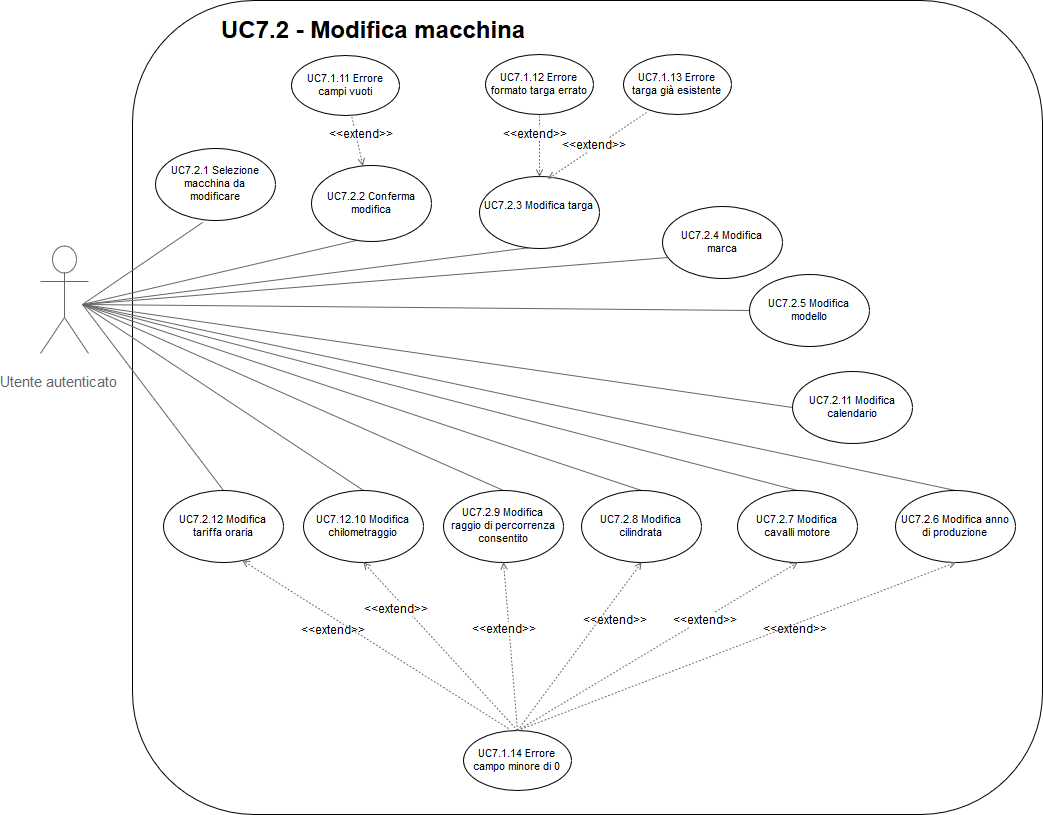
\includegraphics[scale=0.35]{immagini/72.png}    
           \caption{Diagramma UC7.2 - Modifica macchina}
           \end{center}
           \end{figure}  
            
    \newpage
    
    \paragraph{UC 7.3-Eliminazione macchina}
    \begin{itemize}
                \item \textbf{Attori primari}: Utente autenticato;
               
                 \item \textbf{Scopo e descrizione}: L'utente desidera cancellare una o più auto associate al proprio profilo sulla piattaforma;
                 \item \textbf{Scenario principale}: 
                 \begin{itemize}
                     \item L'utente si trova nella sezione dedicata alla cancellazione dell'auto;
                     \item L'utente conferma la cancellazione dell'auto.
                 \end{itemize}
                 \item \textbf{Scenario secondario}: L'utente interrompe il processo e l'eliminazione non viene memorizzata dal sistema.
                 \item \textbf{Precondizione}: L'utente si trova in una schermata in cui è possibile cancellare un auto precedentemente aggiunta;
                 \item \textbf{Postcondizione}: L'utente ha espresso di voler procedere con la cancellazione e quindi il sistema cancella la macchina selezionata.
                 \end{itemize}
                 
          
        
        
    \subsubsection{UC 8-Ricerca macchina}
       \begin{itemize}
        \item \textbf{Attori primari}: Utente autenticato;
        \item \textbf{Attori secondari}: Aws;
        \item \textbf{Scopo e descrizione}: L'utente desidera effettuare un viaggio, pertanto ricerca le auto disponibili sulla piattaforma per percorrere il proprio itinerario.
        \item \textbf{Scenario principale}:
            \begin{itemize}
                \item L'utente ha effettuato l'accesso all'interno del sistema;
                \item L'utente che desidera effettuare la ricerca si posiziona nell'apposita sezione "Cerca".
            \end{itemize}
        
        \item \textbf{Scenario secondario}: L'utente non desidera procedere con la ricerca: smette di compilare i campi richiesti e la ricerca viene interrotta.
       
        
       
        \item \textbf{Precondizione}: L'utente è autenticato all'interno del sistema e si posiziona nella sezione di ricerca.
        \item \textbf{Postcondizione}: L'utente effettua una ricerca e visualizza le offerte di macchine disponibili.
        \end{itemize}
            
      \paragraph{UC 8.1-Inserimento delle zone coperte dal viaggio }
       \begin{itemize}
        \item \textbf{Attori primari}: Utente autenticato;
        
        \item \textbf{Scopo e descrizione}: L'utente autenticato desidera ricercare le auto disponibili per effettuare un viaggio. Per farlo seleziona le aree del viaggio che deve percorrere.
        \item \textbf{Scenario principale}:
            \begin{itemize}
                \item L'utente ha effettuato l'accesso all'interno del sistema;
                \item L'utente che desidera effettuare la ricerca si posiziona nell'apposita sezione "Cerca";
                \item L'utente seleziona le aree che deve percorrere con il suo viaggio.
            \end{itemize}
        
        \item \textbf{Precondizione}: L'utente è autenticato all'interno del sistema e si posiziona nella sezione di ricerca.
        \item \textbf{Postcondizione}: L'utente posizionato nella sezione di ricerca inserisce i dati relativi alle zone del viaggio e il sistema memorizza le scelte.
        \end{itemize}
        
        
        
        
         \paragraph{UC 8.2-Inserimento dei giorni nei quali effettuare il viaggio}
       \begin{itemize}
        \item \textbf{Attori primari}: Utente autenticato;
       
        \item \textbf{Scopo e descrizione}: L'utente autenticato desidera ricercare le auto disponibili per effettuare un viaggio; per farlo seleziona i giorni in cui deve eseguire il viaggio.
        \item \textbf{Scenario principale}:
            \begin{itemize}
                \item L'utente ha effettuato l'accesso all'interno del sistema;
                \item L'utente che desidera effettuare la ricerca si posiziona nell'apposita sezione "Cerca";
                \item L'utente seleziona i giorni in cui deve percorrere con il suo viaggio.
            \end{itemize}
        
        \item \textbf{Precondizione}: L'utente è autenticato all'interno del sistema e si posiziona nella sezione di ricerca.
        \item \textbf{Postcondizione}: L'utente posizionato nella sezione di ricerca inserisce i dati relativi ai giorni in cui vuole svolgere il viaggio e il sistema memorizza le scelte.
        \end{itemize}
        
        
        \paragraph{UC 8.3-Inserimento prezzo massimo desiderato per il viaggio}
       \begin{itemize}
        \item \textbf{Attori primari}: Utente autenticato;
       
        \item \textbf{Scopo e descrizione}: L'utente autenticato desidera ricercare le auto disponibili per effettuare un viaggio; per farlo seleziona il prezzo massimo che vuole pagare per il viaggio.
        \item \textbf{Scenario principale}:
            \begin{itemize}
                \item L'utente ha effettuato l'accesso all'interno del sistema;
                \item L'utente che desidera effettuare la ricerca si posiziona nell'apposita sezione "Cerca";
                \item L'utente seleziona il prezzo che desidera pagare per il viaggio.
            \end{itemize}
        
        \item \textbf{Precondizione}: L'utente è autenticato all'interno del sistema e si posiziona nella sezione di ricerca.
        \item \textbf{Postcondizione}: L'utente posizionato nella sezione di ricerca inserisce i dati relativi al prezzo massimo che desidera pagare per il viaggio e il sistema memorizza le scelte.
        \end{itemize}
        
        
        \paragraph{UC 8.4-Inserimento delle caratteristiche dell'auto con la quale effettuare il viaggio}
       \begin{itemize}
        \item \textbf{Attori primari}: Utente autenticato;
      
        \item \textbf{Scopo e descrizione}: L'utente autenticato desidera ricercare le auto disponibili per effettuare un viaggio; per farlo seleziona le caratteristiche che desidera per l'auto.
        \item \textbf{Scenario principale}:
            \begin{itemize}
                \item L'utente ha effettuato l'accesso all'interno del sistema;
                \item L'utente che desidera effettuare la ricerca si posiziona nell'apposita sezione "Cerca";
                \item L'utente seleziona le caratteristiche volute per l'auto utilizzata per il viaggio.
            \end{itemize}
        
        \item \textbf{Precondizione}: L'utente è autenticato all'interno del sistema e si posiziona nella sezione di ricerca.
        \item \textbf{Postcondizione}: L'utente posizionato nella sezione di ricerca inserisce i dati della macchina da utilizzare per il viaggio e il sistema memorizza le scelte.
        \end{itemize}
        
        
        \paragraph{UC 8.5-Conferma ricerca}
            \begin{itemize}
                \item \textbf{Attori primari}: : Utente autenticato;
                
                \item \textbf{Scopo e descrizione}: L'utente conferma di voler effettuare la ricerca con i dati inseriti precedentemente. 
                \item \textbf{Scenario principale}:
                    \begin{itemize}
                        \item L'utente si trova nella sezione dedicata alla ricerca;
                        \item L'utente conferma l'operazione di ricerca cliccando il pulsante apposito.
                    \end{itemize}
                    \item \textbf{Estensioni}: 
            \begin{itemize}
                \item Nel caso il formato dei campi compilati non sia conforme al formato richiesto viene visualizzato un messaggio di errore (UC 8.6).
            \end{itemize}
                \item \textbf{Precondizione}:L'utente si trova in una schermata in cui è possibile dare la conferma dei dati inseriti su cui eseguire la ricerca;
                \item \textbf{Postcondizione}:L’utente ha espresso di voler procedere con la conferma e quindi con la ricerca all'interno del sistema.
            \end{itemize}
        
        
        
        \paragraph{UC 8.6-Errore formato compilazione campi}
       \begin{itemize}
        \item \textbf{Attori primari}: Utente autenticato;
        \item \textbf{Scopo e descrizione}:  La procedura di ricerca ha riscontrato un errore in merito ai dati inseriti durante la procedura. Nello specifico l'errore è dovuto al fatto che esiste almeno un campo di compilazione con formato non congruo.
        \item \textbf{Scenario principale}:
            \begin{itemize}
                \item L'utente ha effettuato l'accesso all'interno del sistema;
                \item L'utente ha compilato tutti i campi per la ricerca. Almeno uno di questi non è nel formato richiesto, quindi viene scatenato un errore.
            \end{itemize}
        \item \textbf{Precondizione}: L'utente ha compilato i campi di interesse e ha confermato l'operazione. L'utente tenta di effettuare la ricerca inserendo almeno un formato per i campi non consentito.
        \item \textbf{Postcondizione}: L'utente non è in grado di effettuare la ricerca a causa dell'errore scatenato.
        \end{itemize}
  
  \begin{figure}[h!]
           \begin{center}
           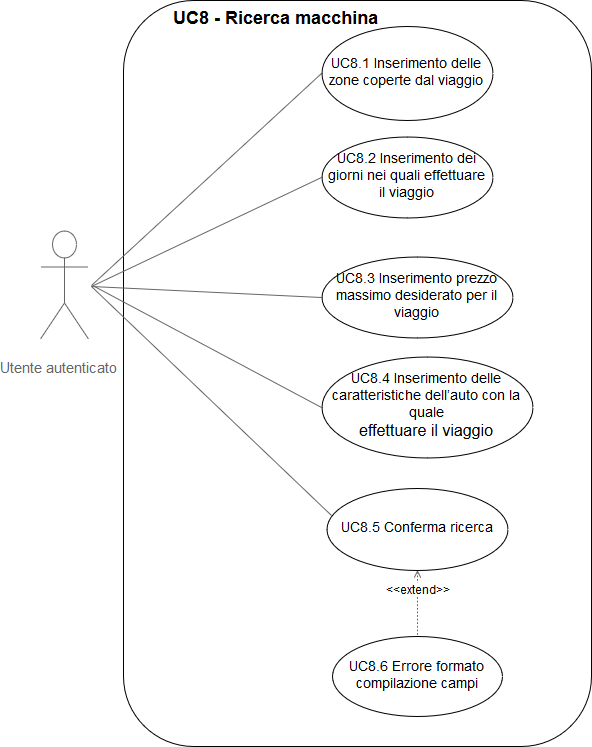
\includegraphics[scale=0.60]{immagini/8.png}    
           \caption{Diagramma UC8 - Ricerca macchina}
           \end{center}
    \end{figure}  
  
  
        
        \subsubsection{UC 9-Prenotazione viaggio}
       \begin{itemize}
        \item \textbf{Attori primari}: Utente autenticato;
        \item \textbf{Attori secondari}: Aws;
        \item \textbf{Scopo e descrizione}: L'utente autenticato desidera prenotare un viaggio utilizzando una delle macchine disponibile per compiere il suo itinerario.
        \item \textbf{Scenario principale}:
            \begin{itemize}
                \item L'utente ha effettuato l'accesso all'interno del sistema;
                \item L'utente ha effettuato una ricerca all'interno del sistema secondo alcuni parametri per ricercare un'auto con cui effettuare un viaggio;
                \item L'utente visualizza i risultati delle macchine che rispondono alle richieste espresse in fase di ricerca da parte dell'utente;
                \item L'utente che desidera effettuare la prenotazione del viaggio seleziona la macchina disponibile che gli interessa;
                \item Una volta selezionata l'utente è in grado di confermare la prenotazione.
            \end{itemize}
        
        \item \textbf{Scenario secondario}: L'utente non desidera procedere con la prenotazione: non seleziona nessuna auto e la prenotazione viene interrotta.
        
        \item \textbf{Precondizione}: L'utente è autenticato all'interno del sistema ed ha effettuato una ricerca. Visualizza i risultati relativi alla ricerca e da qui sceglie una macchina che si adegua alle sue esigenze di viaggio.
        \item \textbf{Postcondizione}: L'utente ha prenotato l'auto per svolgere un determinato viaggio.
        \end{itemize}  
        
        \paragraph{UC 9.1-Selezione macchina}
    \begin{itemize}
                \item \textbf{Attori primari}: Utente autenticato;
                
                 \item \textbf{Scopo e descrizione}: L’utente seleziona una tra le auto che rispondono alla ricerca effettuata;
                 \item \textbf{Scenario principale}: 
                 \begin{itemize}
                     \item L’utente ha effettuato una ricerca per trovare un'auto  con la quale viaggiare all'interno della piattaforma;
                     \item L'utente seleziona una delle macchine che rispondono alla ricerca.
                     \end{itemize}
                 \item \textbf{Precondizione}: L’utente si trova in una schermata che mostra tutti i risultati di una ricerca, nella quale è possibile selezionare una tra le vetture con la quale effettuare il viaggio;
                 \item \textbf{Postcondizione}: L’utente seleziona l'auto sulla quale vuole effettuare la prenotazione del viaggio.
                 \end{itemize}
                 
        \paragraph{UC 9.2-Conferma prenotazione}
            \begin{itemize}
                \item \textbf{Attori primari}: Utente autenticato;
                
                \item \textbf{Scopo e descrizione}: L'utente conferma di voler effettuare la prenotazione della macchina precedentemente selezionata. 
                \item \textbf{Scenario principale}:
                    \begin{itemize}
                        \item L'utente si trova nella sezione dedicata alla macchina selezionata;
                        \item L'utente conferma l'operazione di prenotazione cliccando il pulsante apposito.
                    \end{itemize}
                \item \textbf{Precondizione}:L'utente si trova in una schermata in cui è possibile dare la conferma della prenotazione dell'auto precedentemente selezionata dopo la fase di ricerca;
                \item \textbf{Postcondizione}:L’utente ha espresso di voler procedere con la conferma e quindi il sistema memorizza la prenotazione del viaggio.
            \end{itemize}
            
            \begin{figure}[h!]
           \begin{center}
           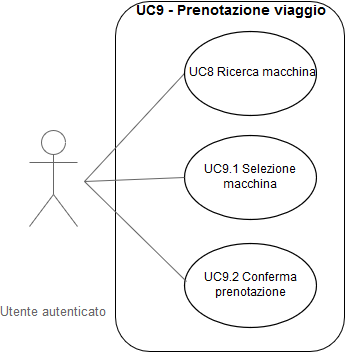
\includegraphics[scale=0.60]{immagini/9.png}    
           \caption{Diagramma UC9 - Prenotazione viaggio}
           \end{center}
            \end{figure}  
                  
            
       
     
       \subsubsection{UC 10-Recensione esperienza viaggio}
       \begin{itemize}
        \item \textbf{Attori primari}: Utente autenticato;
        \item \textbf{Attori secondari}: Aws;
        \item \textbf{Scopo e descrizione}: L'utente autenticato desidera recensire un viaggio che ha effettuato precedentemente.
        \item \textbf{Scenario principale}:
            \begin{itemize}
                \item L'utente ha effettuato l'accesso all'interno del sistema;
                \item L'utente a seguito di una ricerca ha scelto una macchina con la quale ha effettuato un viaggio;
                \item L'utente ha terminato il suo viaggio e visualizza una schermata in cui è possibile lasciare una recensione sul viaggio appena effettuato.
            \end{itemize}
        
        \item \textbf{Scenario secondario}: L'utente non desidera procedere con la recensione: la recensione non viene memorizzata dal sistema.
       
        
        \item \textbf{Precondizione}: L'utente è autenticato all'interno del sistema ed ha effettuato e concluso un viaggio. L'utente è quindi in grado di visualizzare una schermata in cui è in grado di recensire un viaggio che ha appena effettuato.
        \item \textbf{Postcondizione}: L'utente ha recensito l'esperienza di viaggio che ha concluso, ottenendo i premi previsti per la gamification all'interno dell'app.
        \end{itemize}  
      
      
       \subsubsection{UC 11: Chiusura del viaggio}
  
        \begin{itemize}
        \item \textbf{Attori primari}: Utente autenticato;
        \item \textbf{Attori secondari}: Aws;
        \item \textbf{Scopo e descrizione}: L'utente che ha effettuato un viaggio conferma di voler chiudere; 
        \item \textbf{Scenario principale}:
            \begin{itemize}
                \item L'utente è autenticato all'interno della piattaforma;
                \item L'utente sta effettuando un viaggio
                \item L'utente desidera terminare il viaggio e quindi sceglie la funzionalità "Termina";
                \item L'utente conferma la terminazione del viaggio;
            \end{itemize}
         
        \item \textbf{Inclusioni}:
             \begin{itemize}
                \item L'utente conferma la conclusione del viaggio (UC 11.1);
            \end{itemize}
        \item \textbf{Precondizione}: L'utente è riconosciuto nel sistema e sta effettuando correntemente un viaggio previa prenotazione;
        \item \textbf{Postcondizione}: L'utente conclude il viaggio e visualizza una schermata riassuntiva con possibilità di recensire.
        \end{itemize}


        \paragraph{UC 11.1:Conferma chiusura viaggio}
            \begin{itemize}
                \item \textbf{Attori primari}: Utente autenticato;
                
                \item \textbf{Scopo e descrizione}: L'utente conferma di voler effettuare la terminazione del viaggio che sta effettuando; 
                \item \textbf{Scenario principale}:
                    \begin{itemize}
                        \item L'utente si trova nella dashboard dedicata ai dati relativi al viaggio;
                        \item L'utente conferma l'operazione di terminazione del viaggio cliccando il pulsante apposito.
                    \end{itemize}
                \item \textbf{Precondizione}:L'utente si trova in una schermata in cui è possibile dare la conferma
                del termine del viaggio;
                \item \textbf{Postcondizione}:L’utente ha espresso di voler procedere con la terminazione del viaggio e quindi la procedura si conclude.
            \end{itemize}
        

        
            
       \subsubsection{UC 12-Visualizzazione dati personali relativi all'utente}  
      \begin{itemize}
        \item \textbf{Attori primari}: Utente autenticato;
        \item \textbf{Attori secondari}: Aws;
        \item \textbf{Scopo e descrizione}: L'utente visualizza i dati personali come nome, cognome, mail, username, dati opzionali e recensioni relativi al proprio account; 
        \item \textbf{Scenario principale}: L'utente autenticato richiede al sistema di visualizzare i propri dati personali;
        \item \textbf{Precondizione}: L'utente autenticato si trova nella propria area personale;
        \item \textbf{Postcondizione}: L'utente autenticato ottiene la visualizzazione dei dati personali.
        \end{itemize}  
        
     
        
      \subsubsection{UC 13-Visualizzazione dati relativi alle macchine messe a disposizione dall'utente}
        \begin{itemize}
        \item \textbf{Attori primari}: Utente autenticato;
        \item \textbf{Attori secondari}: Aws;
        \item \textbf{Scopo e descrizione}: L'utente visualizza una lista con le auto messe a disposizione da lui, visualizzando per ogni auto le varie caratteristiche; 
        \item \textbf{Scenario principale}: L'utente richiede al sistema di visualizzare le proprie auto;
        \item \textbf{Precondizione}: L'utente si trova nella propria area personale;
        \item \textbf{Postcondizione}: L'utente visualizza una lista con le sue auto messe a disposizione.
        \end{itemize}
 
            
         \subsubsection{UC 14-Visualizzazione itinerari compiuti dall'utente}
        \begin{itemize}
        \item \textbf{Attori primari}: Utente autenticato;
        \item \textbf{Attori secondari}: Aws;
        \item \textbf{Scopo e descrizione}: L'utente visualizza una lista con i viaggi compiuti, visualizzando per ogni viaggio, luogo di partenza, orario di partenza, luogo di arrivo, orario di arrivo, distanza percorsa, fattura; 
        \item \textbf{Scenario principale}: L'utente richiede al sistema di visualizzare gli itinerari compiuti;
        \item \textbf{Precondizione}: L'utente si trova nella propria area personale;
        \item \textbf{Postcondizione}: L'utente visualizza una lista con gli itinerari compiuti, o se in mancanza di tali mostrerà una schermata vuota.
        \end{itemize}    
            
 
        \subsubsection{UC 15-Visualizzazione del profilo di un altro utente}
        \begin{itemize}
            \item  \textbf{Attori primari}: Utente autenticato;
            \item \textbf{Attori secondari}: Aws;
            \item \textbf{Scopo e descrizione}: L'utente desidera avere più informazioni su un utente.
            \item \textbf{Scenario principale}: L'utente visualizza il profilo di un altro utente.
            \item \textbf{Precondizione}: L'utente è autenticato;
            \item \textbf{Postcondizione}: Il sistema ha elaborato la richiesta e presenta una schermata contenente le informazioni dell'utente
        \end{itemize}   
  
        
        
    \subsubsection{UC 16-Visualizzazione statistiche personali}  
      \begin{itemize}
        \item \textbf{Attori primari}: Utente autenticato;
        \item \textbf{Attori secondari}: Aws;
        \item \textbf{Scopo e descrizione}: L'utente visualizza i dati personali relativi alle proprie statistiche relative al suo utilizzo dell'applicazione. I dati visualizzabili in questa sezione precisamente sono:
            \begin{itemize}
                \item Stato di avanzamento dell'utente in termini di punti rank e badge;
                \item Visualizzazione statistiche azioni fatte all'interno dell'applicazione: numero viaggi, numero prenotazioni, km medi effettuati per viaggio;
                \item Missioni conclusioni, da fare, visualizzare missioni giornaliere sbloccate;
                \item Visualizzazione badge ottenuti.
            \end{itemize}
        \item \textbf{Scenario principale}: L'utente autenticato richiede al sistema di visualizzare i propri dati personali relativi alle statistiche di utilizzo dell'applicazione;
        \item \textbf{Precondizione}: L'utente autenticato si trova nella propria area personale;
        \item \textbf{Postcondizione}: L'utente autenticato ottiene la visualizzazione dei dati personali relativi alle statistiche di utilizzo dell'applicazione.
        \end{itemize}  
  
    \subsubsection{UC 17-Visualizzazione classifiche generali}  
      \begin{itemize}
        \item \textbf{Attori primari}: Utente autenticato;
        \item \textbf{Attori secondari}: Aws;
        \item \textbf{Scopo e descrizione}: L'utente visualizza i dati personali relativi alle classifiche generali calcolate dalla piattaforma. Le classifiche in questa sezione precisamente sono:
            \begin{itemize}
                \item Classifica globale assoluta sulla base dei punti rank degli utenti della piattaforma. La classifica è calcolata su scala decrescente: tanti più punti un utente possiede tanto più alta sarà la sua posizione;
                \item Classifica globale mensile sulla base dei punti rank degli utenti della piattaforma. Il posizionamento degli utenti è calcolato nello stesso modo della scala assoluta, solamente che vengono conteggiati esclusivamente i punti acquisiti su base mensile, non assoluta.
            \end{itemize}
            
        \item \textbf{Scenario principale}: L'utente autenticato richiede al sistema di visualizzare i dati personali relativi alle classifiche interne all'applicazione;
        \item \textbf{Precondizione}: L'utente è autenticato nel sistema;
        \item \textbf{Postcondizione}: L'utente autenticato ottiene la visualizzazione delle classifiche interne all'applicazione.
        \end{itemize}  
     
         
        
        
    \subsubsection{UC 18-Visualizzazione buoni spesa personali}  
      \begin{itemize}
        \item \textbf{Attori primari}: Utente autenticato;
        \item \textbf{Attori secondari}: Aws;
        \item \textbf{Scopo e descrizione}: L'utente visualizza i dati personali relativi ai buoni spesa (ovvero buoni sconto utilizzabili in aziende partner alla piattaforma) ottenuti/ottenibili/da riscuotere/riscossi dall'utente.
        \item \textbf{Scenario principale}: L'utente autenticato richiede al sistema di visualizzare i buoni spesa relativi all'utente;
        \item \textbf{Precondizione}: L'utente è autenticato nel sistema;
        \item \textbf{Postcondizione}: L'utente autenticato ottiene la visualizzazione dei buoni sconto che la piattaforma offre.
        \end{itemize}
  
    
            
    \subsubsection{UC 19-Riscuoti buono}  
      \begin{itemize}
        \item \textbf{Attori primari}: Utente autenticato;
        \item \textbf{Attori secondari}: Aws;
        \item \textbf{Scopo e descrizione}: L'utente intende utilizzare il buono sconto da lui cumulato presso aziende partner alla piattaforma. Con l'azione di riscossione notifica la sistema che ha utilizzato il buono disponibile, pertanto tale buono non è più utilizzabile in futuro.
        \item \textbf{Scenario principale}:
            \begin{itemize}
                \item L'utente autenticato si trova nella sezione di visualizzazione da buoni da lui cumulati;
                \item L'utente seleziona un buono tra quelli che ha cumulato;
                \item L'utente l'utente esprime la volontà di utilizzare il buono utilizzato
                
            \end{itemize}
            
        \item \textbf{Scenario secondario}: L'utente non intende proseguire con l'utilizzo del buono, l'azione non viene memorizzata nel sistema
         \item \textbf{Inclusioni}:
            \begin{itemize}
                \item L'utente seleziona il buono da utilizzare (UC 19.1);
                \item L'utente conferma di voler usufruire del buono da lui disposto(UC 19.2).
            \end{itemize}
          
        \item \textbf{Precondizione}: L'utente è autenticato nel sistema, si trova nella sezione di visualizzazione dei buoni e ha a disposizione almeno un buono da utilizzare;
        \item \textbf{Postcondizione}: L'utente autenticato usufruisce del buono spesa da lui posseduto.
        \end{itemize}  
        
            
    \subparagraph{UC 19.1-Selezione buono di cui usufruire}
    \begin{itemize}
                \item \textbf{Attori primari}: Utente autenticato;
                
                 \item \textbf{Scopo e descrizione}: L’utente seleziona uno tra i buoni a lui a disposizione per poterne usufruire;
                 \item \textbf{Scenario principale}: 
                 \begin{itemize}
                     \item L’utente si trova nella sezione dedicata alla visualizzazione dei buoni disponibili;
                     \item L'utente seleziona uno tra i buoni disponibili del quale vuole usufruire.          \end{itemize}
                 \item \textbf{Precondizione}: L’utente si trova in una schermata in cui è possibile selezionare il buono su cui si vuole riscuotere uno sconto;
                 \item \textbf{Postcondizione}: L’utente seleziona il buono che intende utilizzare.
                 \end{itemize}
    
    \subparagraph{UC 19.2-Conferma riscossione buono}
    \begin{itemize}
                \item \textbf{Attori primari}: Utente autenticato;
               
                 \item \textbf{Scopo e descrizione}: L’utente conferma di voler riscuotere il buono sconto precedentemente utilizzato per permettere al sistema di memorizzare la scelta;
                 \item \textbf{Scenario principale}: 
                 \begin{itemize}
                     \item L’utente si trova nella sezione dedicata alla riscossione dei buoni a lui disponibili;
                     \item L'utente conferma l'operazione di riscossione del buono cliccando il pulsante apposito. 
                 \end{itemize}
                 \item \textbf{Precondizione}: L’utente si trova in una schermata in cui è possibile dare la conferma dell'operazione di riscossione;
                 \item \textbf{Postcondizione}: L’utente ha espresso di voler procedere con la riscossione del buono.
                 \end{itemize}
                   
    \begin{figure}[h!]
           \begin{center}
           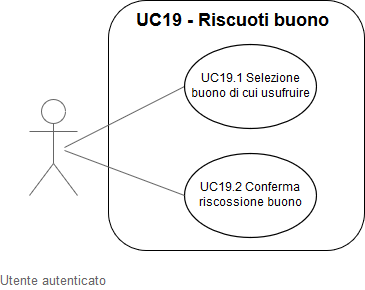
\includegraphics[scale=0.50]{immagini/19.png}    
           \caption{Diagramma UC19 - Riscuoti buono}
           \end{center}
            \end{figure}  
   
     
               
       \subsubsection{UC 20-Visualizzazione sezione esplora}  
      \begin{itemize}
        \item \textbf{Attori primari}: Utente autenticato;
        \item \textbf{Attori secondari}: Aws;
        \item \textbf{Scopo e descrizione}: L'utente visualizza i dati relativi alla sezione "esplora", all'interno della quale l'utente può visualizzare offerte relative alla zona in cui risiede, quali promozioni temporanee in partnership con aziende.
            
        \item \textbf{Scenario principale}: L'utente autenticato richiede al sistema di visualizzare la sezione dell'applicazione "esplora";
        \item \textbf{Precondizione}: L'utente è autenticato nel sistema;
        \item \textbf{Postcondizione}: L'utente autenticato ottiene la visualizzazione della sezione esplora.
        \end{itemize}        
     
                 
        \subsubsection{UC 21-Visualizzazione ruota dei premi}  
      \begin{itemize}
        \item \textbf{Attori primari}: Utente autenticato;
        \item \textbf{Attori secondari}: Aws;
        \item \textbf{Scopo e descrizione}: L'utente che visualizza la ruota della fortuna ha la possibilità di ricevere dei premi quando si ferma.
           
            
        \item \textbf{Scenario principale}: L'utente autenticato accede per la prima volta nella giornata nell'applicazione, visualizza la ruota della fortuna che consente di ricevere premi all'interno dell'applicazione, la ferma ed eventualmente riceve un premio;
        \item \textbf{Precondizione}: L'utente è autenticato nel sistema;
        \item \textbf{Postcondizione}: L'utente autenticato ottiene la visualizzazione della ruota della fortuna.
        \end{itemize}  
      
 
    
        
         
    
        
        
           
        
        
       

    
    